\documentclass[11pt]{article}
\usepackage[margin=0.88in]{geometry}
\usepackage{amsmath,amssymb,amsfonts,amsthm,mathtools}
\usepackage{booktabs,longtable,array,enumitem,graphicx,xcolor,hyperref,cleveref}
\usepackage{listings}
\usepackage{tikz}
\usetikzlibrary{arrows.meta,positioning,shapes.geometric,fit,calc}
\hypersetup{colorlinks=true,linkcolor=blue!50!black,citecolor=blue!50!black,urlcolor=blue!50!black}
\definecolor{darkblue}{RGB}{28,74,126}
\definecolor{darkgreen}{RGB}{25,110,76}
\definecolor{darkred}{RGB}{140,45,45}
\definecolor{softgray}{RGB}{246,247,250}
\definecolor{softblue}{RGB}{235,243,252}
\definecolor{softgreen}{RGB}{236,248,241}
\newtheorem{definition}{Definition}[section]
\newtheorem{assumption}[definition]{Assumption}
\newtheorem{theorem}[definition]{Theorem}
\newtheorem{proposition}[definition]{Proposition}
\newtheorem{lemma}[definition]{Lemma}
\newtheorem{corollary}[definition]{Corollary}
\newtheorem{example}[definition]{Example}
\newtheorem{remark}[definition]{Remark}
\newcommand{\R}{\mathbb{R}}
\newcommand{\N}{\mathbb{N}}
\newcommand{\Z}{\mathbb{Z}}
\newcommand{\T}{\mathbb{T}}
\newcommand{\E}{\mathbb{E}}
\newcommand{\calG}{\mathcal{G}}
\newcommand{\calD}{\mathcal{D}}
\newcommand{\calC}{\mathcal{C}}
\newcommand{\calB}{\mathcal{B}}
\newcommand{\calX}{\mathcal{X}}
\newcommand{\calY}{\mathcal{Y}}
\newcommand{\calM}{\mathcal{M}}
\newcommand{\calN}{\mathcal{N}}
\newcommand{\calP}{\mathcal{P}}
\newcommand{\calL}{\mathcal{L}}
\newcommand{\calR}{\mathcal{R}}
\newcommand{\calS}{\mathcal{S}}
\newcommand{\calK}{\mathcal{K}}
\newcommand{\calF}{\mathcal{F}}
\newcommand{\calA}{\mathcal{A}}
\newcommand{\calH}{\mathcal{H}}
\newcommand{\calU}{\mathcal{U}}
\newcommand{\calV}{\mathcal{V}}
\newcommand{\calW}{\mathcal{W}}
\newcommand{\calZ}{\mathcal{Z}}
\newcommand{\oplusT}{\oplus_{\rm trop}}
\newcommand{\odotT}{\odot_{\rm trop}}
\newcommand{\argmax}{\operatorname*{arg\ max}}
\newcommand{\argmin}{\operatorname*{arg\ min}}
\newcommand{\softmax}{\operatorname{softmax}}
\newcommand{\LSE}{\operatorname{LSE}}
\newcommand{\diag}{\operatorname{diag}}
\newcommand{\dist}{\operatorname{dist}}
\newcommand{\rank}{\operatorname{rank}}
\newcommand{\Span}{\operatorname{span}}
\newcommand{\Conv}{\operatorname{Conv}}
\newcommand{\bits}{\operatorname{bits\mbox{-}per\mbox{-}byte}}
\newcommand{\norm}[1]{\left\lVert #1\right\rVert}
\newcommand{\abs}[1]{\left\lvert #1\right\rvert}
\newcommand{\ip}[2]{\left\langle #1,#2\right\rangle}
\newcommand{\trans}{^{\mathsf T}}
\newcommand{\eps}{\varepsilon}
\lstset{basicstyle=\ttfamily\small,breaklines=true,columns=fullflexible,frame=single,backgroundcolor=\color{softgray}}
\setlist[itemize]{leftmargin=1.3em,itemsep=2pt,topsep=2pt}
\setlist[enumerate]{leftmargin=1.5em,itemsep=2pt,topsep=2pt}
\sloppy

\title{\vspace{-2em}\textbf{TropicalGT: Tropical Attention, Polyhedral Reasoning, and Bits-per-byte-Safe Training for Graph-Token Reasoning Agents}}
\author{Amelie Schreiber}
\date{June 2026}

\begin{document}
\maketitle

\begin{abstract}
Tropical Attention, introduced at NeurIPS 2025 by Hashemi, Pasque, Teska, and Yoshida, replaces softmax-normalized dot-product attention with a max-plus, tropical-projective attention mechanism designed for neural algorithmic reasoning.  The central insight is that many dynamic-programming and combinatorial-optimization value functions are tropical polynomials: maxima of affine functions, or compositions of max and ordinary addition.  This paper develops \emph{TropicalGT}, a graph-token and reasoning-agent architecture that turns that first iteration into a broader training theory.  TropicalGT uses tropical attention heads as hard, auditable routing primitives; graph-token transformers as equivariant carriers of typed reasoning states; blockwise ring evaluation as a long-context execution schedule; tropical Newton polytopes as diagnostics of active proof alternatives; and bits-per-byte-gated objectives as the deployment contract.  The goal is not merely to replace softmax.  The goal is to make hidden reasoning trajectories behave like stable polyhedral algorithms whose active faces, margins, certificates, and compression utility can be inspected.

We give a rigorous mathematical specification of TropicalGT, including definitions of tropicalized token spaces, multi-head tropical graph attention, Hilbert-metric scores, active-face certificates, blockwise tropical scans, and structured reasoning packets.  We prove equivariance, 1-Lipschitz stability, active-face preservation under quantization, exactness of blockwise max-plus evaluation, simulation theorems for dynamic-programming recurrences, and a conditional-information theorem explaining when tropical certificates can improve held-out bits-per-byte.  We then propose training losses, metrics, regularizers, and curricula for algorithmic tasks, graph reasoning, retrieval, long-context reasoning, memory compression, and behavior control.  The paper includes implementation-level pseudocode, PyTorch-style kernel sketches, dataset and ablation protocols, and reproducibility details.  It is written as a research-program paper: the formal theorems hold under explicit finite or compact assumptions, while empirical claims are framed as hypotheses to be validated by matched ablations and score-first bits-per-byte evaluation.
\end{abstract}

\tableofcontents
\newpage

\section{Motivation and relation to the ToricGT program}

ToricGT began with graph-token reasoning, tropical ring attention, noncommutative-torus phase channels, finite toric or BGG certificates, and a strict compression contract: auxiliary structure is useful only when it improves held-out bits-per-byte, reasoning quality, retrieval quality, behavior control, or another predeclared metric after artifact-byte accounting.  The original ToricGT formulation already treated max-plus heads as dynamic-programming primitives, and later iterations developed full-context reasoning, filtered persistence complexes, sheaves, vector bundles, derived objects, MCP memory, graph-structured vector retrieval, and oracle trajectory classifiers.  TropicalGT isolates and expands the tropical component of that program.

The NeurIPS 2025 Tropical Attention paper supplies the catalyst.  Its central claim is that softmax attention is geometrically misaligned with combinatorial algorithms: softmax produces smooth mixtures, while dynamic programs often require decisive max/min selections over polyhedral value functions.  Tropical Attention addresses this by moving attention into tropical projective space, scoring query-key agreement by a tropical Hilbert metric, aggregating by max-plus matrix-vector products, and returning the result to Euclidean coordinates for ordinary transformer processing \cite{hashemi2025tropical}.  The authors prove that multi-head Tropical Attention can approximate tropical circuits and simulate max-plus dynamic programs; the official OpenReview record lists it as a NeurIPS 2025 poster and states that MHTA stacks approximate tropical circuits and realize tropical transitive closure with polynomial resource bounds \cite{hashemi2025openreview}.  The public code repository exposes a standalone \texttt{TropicalAttention.py} kernel, experimental scripts, and eleven combinatorial task generators \cite{hashemi2025code}.

TropicalGT also builds on the tropical expressivity program of Su and Liu, where zero-temperature self-attention is analyzed as a tropical rational map whose query-space cells are power diagrams and whose multi-head complexity is governed by Minkowski sums of Newton polytopes \cite{su2026expressivity}.  The TokenGT expressivity extension sharpens this picture for graph data: graph tokenization changes the effective token count, makes vertex-edge incidence directly visible to attention, supports graph-to-graph universality on bounded domains, and clarifies the Boolean-circuit and toric-boundary edge cases \cite{schreiber2026tokengtexpressivity}.  TropicalGT-I turns those expressivity claims into a training and audit contract: the code logs supports, margins, structural certificates, GFlowNet paths, GraphCG directions, and filtered simplicial objects rather than treating the tropical skeleton as an invisible proof device.

TropicalGT asks the next question: what happens if tropical attention is not a local replacement for softmax, but the organizing principle for an auditable reasoning-agent stack?  The answer is a model class with five layers:
\begin{enumerate}
\item \textbf{Tropical kernels.}  Selected attention heads operate over max-plus or min-plus semirings, exposing active supports, top-two margins, and polyhedral cells.
\item \textbf{Graph-token carriers.}  Nodes, edges, memory records, proof obligations, tool calls, and retrieved evidence become typed graph tokens processed equivariantly.
\item \textbf{Polyhedral diagnostics.}  The active affine candidates of a tropical head form Newton polytopes and normal-fan cells; reasoning decisions become active faces.
\item \textbf{Certificate-aware training.}  Dynamic-programming recurrences, shortest-path trees, subset-sum tables, proof graphs, persistence summaries, and behavior labels are converted into finite certificates and losses.
\item \textbf{Bits-per-byte deployment.}  Tropical probes may remain teacher-side.  They enter the deployable student only when quantized export improves held-out bits-per-byte or gives a predeclared reasoning/control gain without statistically meaningful compression regression.
\end{enumerate}

The paper is also a response to a practical difficulty in reasoning-agent training.  Many models can output plausible intermediate reasoning, but hidden trajectories are rarely audited.  Tropical structure gives an intermediate language between symbolic proof and opaque activation.  A tropical head computes a maximum; the maximizing index is a discrete certificate.  If the top-two margin is large, the certificate is stable.  If the same certificate recurs across graph isomorphisms or value shifts, it is evidence of algorithmic structure.  If the certificate improves future-byte prediction or verifier accuracy under strict prefix dependence, it has compression value.

\paragraph{Contributions.}
This paper contributes:
\begin{enumerate}
\item a self-contained formalization of TropicalGT as a graph-token transformer with tropical, softmax, hybrid, and ring-evaluated attention heads;
\item an exact mathematical dictionary from tropical attention to active faces, normal fans, dynamic-programming recurrences, and reasoning certificates;
\item theorems for equivariance, stability, active-face preservation, tropical circuit simulation, graph recurrence simulation, and bits-per-byte utility of prefix-visible certificates;
\item a practical catalogue of losses, metrics, objectives, and regularizers for training TropicalGT on algorithmic reasoning, graph reasoning, long-context retrieval, and behavior-controlled reasoning;
\item implementation details, pseudocode, reproducibility protocols, and ablation ladders designed to separate real compression/reasoning gain from ornamental mathematical structure.
\end{enumerate}

\begin{figure}[h]
\centering
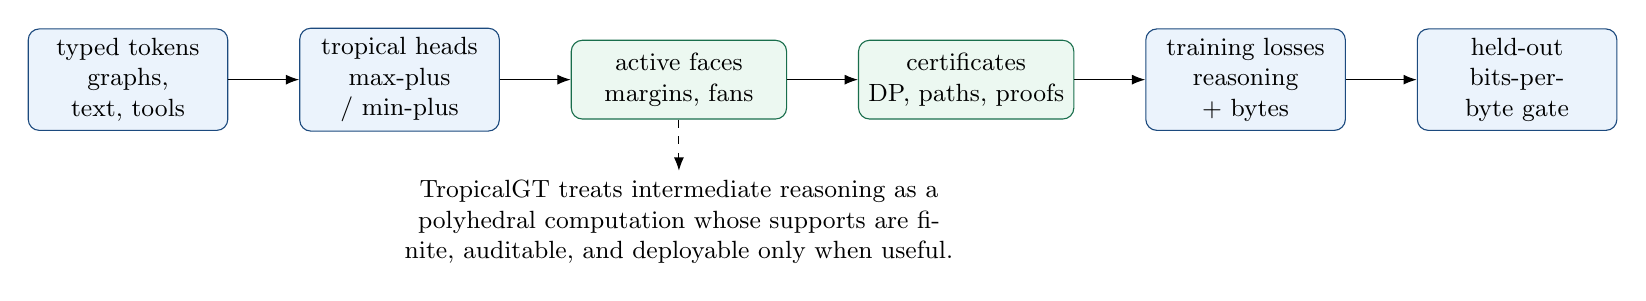
\begin{tikzpicture}[node distance=0.9cm,>=Latex, every node/.style={font=\small}]
\tikzstyle{box}=[rounded corners, draw=darkblue, fill=softblue, minimum height=1.0cm, text width=2.3cm, align=center]
\tikzstyle{gbox}=[rounded corners, draw=darkgreen, fill=softgreen, minimum height=1.0cm, text width=2.5cm, align=center]
\node[box] (input) {typed tokens\\graphs, text, tools};
\node[box, right=of input] (trop) {tropical heads\\max-plus / min-plus};
\node[gbox, right=of trop] (poly) {active faces\\margins, fans};
\node[gbox, right=of poly] (cert) {certificates\\DP, paths, proofs};
\node[box, right=of cert] (train) {training losses\\reasoning + bytes};
\node[box, right=of train] (gate) {held-out\\bits-per-byte gate};
\draw[->] (input)--(trop); \draw[->] (trop)--(poly); \draw[->] (poly)--(cert); \draw[->] (cert)--(train); \draw[->] (train)--(gate);
\node[below=0.65cm of poly, text width=8.0cm, align=center] (cap) {TropicalGT treats intermediate reasoning as a polyhedral computation whose supports are finite, auditable, and deployable only when useful.};
\draw[->, dashed] (poly) -- (cap);
\end{tikzpicture}
\caption{TropicalGT pipeline.  Tropical heads expose active maximizers and margins; these become finite certificates and training losses; deployment is controlled by held-out bits-per-byte and reasoning metrics.}
\end{figure}

\section{Review of Tropical Attention and its limitations}

\subsection{The first iteration: tropical attention at NeurIPS 2025}

The Tropical Attention paper is motivated by neural algorithmic reasoning.  Dynamic programming algorithms for combinatorial optimization frequently combine max/min with ordinary addition.  In the max-plus semiring, a recurrence such as
\begin{equation}
D_{t+1}(v)=\max_{u\to v}\{D_t(u)+w(u,v)\}
\end{equation}
is linear: addition in the semiring is maximum, multiplication is ordinary addition.  The value function is a tropical polynomial, i.e. a maximum of affine monomials.  This matches the polyhedral geometry of optimal alternatives.  The paper contrasts this with softmax dot-product attention, where every key receives positive mass and sharp choices are smoothed.  The arXiv version states that Tropical Attention operates natively in the max-plus semiring and is intended to preserve sharp, scale-invariant reasoning that softmax blurs \cite{hashemi2025tropical}.

The mechanism has four conceptual steps:
\begin{enumerate}
\item map Euclidean token embeddings to tropical projective coordinates by a valuation-like map;
\item form tropical linear projections for queries, keys, and values;
\item compute query-key agreement using the tropical Hilbert projective metric;
\item aggregate values by a tropical matrix-vector product and devaluate back to Euclidean coordinates.
\end{enumerate}

The paper's public slides summarize the key attention equation as a projective selection: the tropical context picks the value that best aligns projectively with the query using a Hilbert distance and a max-plus reduction \cite{hashemi2025slides}.  It also emphasizes three requirements for algorithmic alignment: hard argmax/argmin operations, piecewise-linear decision boundaries, and robustness to perturbations.  Those are exactly the properties TropicalGT makes explicit and auditable.

\subsection{What TropicalGT changes}

The first iteration proves that tropical attention can simulate tropical circuits and performs well on controlled algorithmic tasks.  TropicalGT adds five extensions.

First, it treats tropical attention as one head family inside a graph-token model.  Some heads should remain softmax because natural-language and diffuse semantic retrieval sometimes require mixture.  TropicalGT uses a typed head bank: tropical heads for algorithmic max/min, softmax heads for distributional semantics, and hybrid heads when the model must learn a soft-to-hard curriculum.

Second, it makes the active maximizer a first-class supervision object.  The Tropical Attention paper visualizes sharp attention maps for Quickselect and Knapsack; TropicalGT trains on the support itself when a certificate is available.  The support is not merely an explanation.  It is a discrete variable whose entropy, stability, and agreement with a teacher can be measured.

Third, it uses tropical geometry beyond max-plus arithmetic.  A head with affine candidates \(a_r\cdot h+b_r\) has a lifted Newton polytope \(\Conv(a_r,b_r)\).  The hidden state \(h\) exposes a face of this polytope.  The corresponding normal fan partitions hidden space into decision cells.  The full TropicalGT geometric program records active faces, wall distances, and bends when fan geometry is available; the v1 implementation logs active supports, top-two margins, support entropies, and margin-threshold wall-hit proxies as certificate diagnostics.

Fourth, it connects tropical attention to reasoning trajectories and long context.  A tropical head can be evaluated blockwise because maximum is associative and commutative.  This gives exact support scans over large context shards.  For long-context reasoning, the support of a tropical query over evidence blocks is a compact proof-of-use certificate.

Fifth, it retains the ToricGT compression contract.  Every tropical loss is staged.  Audit-only probes come first; loss-enabled probes require exact/surrogate agreement; deployed probes must improve held-out bits-per-byte or predeclared reasoning/control metrics after artifact accounting.

\subsection{Limitations inherited from the source paper}

The Tropical Attention paper itself notes that its experiments were on combinatorial algorithms and had not yet demonstrated scale to generative autoregressive language tasks; it also flags computational and memory overhead from tropical operations and the Hilbert metric \cite{hashemi2025tropical}.  TropicalGT treats those as design constraints:
\begin{itemize}
\item use tropical heads selectively, not universally;
\item implement max-plus kernels with blockwise scans and sparsity masks;
\item train on algorithmic and graph-structured slices before mixing into natural text;
\item distill tropical support codes into compact students;
\item report bits-per-byte and artifact bytes, not only task accuracy.
\end{itemize}

\section{Mathematical foundations}

\subsection{The tropical semiring and tropical polynomials}

\begin{definition}[Max-plus semiring]
The max-plus tropical semiring is
\begin{equation}
\T_{\max}=\R\cup\{-\infty\},\qquad a\oplusT b=\max(a,b),\qquad a\odotT b=a+b.
\end{equation}
The additive identity is \(-\infty\) and the multiplicative identity is \(0\).  Matrix multiplication over \(\T_{\max}\) is
\begin{equation}
(A\odotT B)_{ij}=\max_k(A_{ik}+B_{kj}).
\end{equation}
The min-plus semiring is obtained by replacing maximum with minimum and using \(+\) as multiplication.
\end{definition}

\begin{definition}[Tropical polynomial]
A tropical polynomial in \(x\in\R^d\) is a function
\begin{equation}
f(x)=\bigoplus_{r=1}^R c_r\odotT x_1^{\odotT \alpha_{r1}}\odotT\cdots\odotT x_d^{\odotT \alpha_{rd}}
     =\max_{1\le r\le R}\{c_r+\ip{\alpha_r}{x}\},
\end{equation}
where \(c_r\in\R\) and \(\alpha_r\in\N^d\).  Thus tropical polynomials are convex piecewise-linear functions.  The active set at \(x\) is
\begin{equation}
A_f(x)=\argmax_r\{c_r+\ip{\alpha_r}{x}\}.
\end{equation}
\end{definition}

\begin{lemma}[Tropical polynomials are 1-Lipschitz with respect to coefficient perturbation]
Let
\(f(x)=\max_r(c_r+\ip{\alpha_r}{x})\) and \(g(x)=\max_r(d_r+\ip{\alpha_r}{x})\).  If \(\max_r|c_r-d_r|\le \eps\), then \(|f(x)-g(x)|\le \eps\) for all \(x\).
\end{lemma}
\begin{proof}
For each \(r\), \(c_r+\ip{\alpha_r}{x}\le d_r+\ip{\alpha_r}{x}+\eps\).  Taking maxima gives \(f(x)\le g(x)+\eps\).  Reversing the roles of \(c\) and \(d\) gives \(g(x)\le f(x)+\eps\).  The result follows.
\end{proof}

\subsection{Tropical projective space and Hilbert metric}

Tropical attention uses projective invariance: adding a constant to every coordinate of a vector should not change its meaning.  Let \({\bf 1}=(1,\ldots,1)\).  Two vectors \(x,y\in\R^d\) are tropically projectively equivalent if \(x-y=\lambda {\bf 1}\) for some scalar \(\lambda\).  The quotient \(\R^d/\R{\bf 1}\) is tropical projective space.  A convenient section is
\begin{equation}
\pi(x)=x-\max_i x_i\, {\bf 1},\qquad \max_i \pi(x)_i=0.
\end{equation}
The tropical Hilbert projective metric is
\begin{equation}
d_H(x,y)=\max_i(x_i-y_i)-\min_i(x_i-y_i).
\end{equation}
It is invariant under adding constants to either argument.

\begin{lemma}[Projective invariance]
For any \(x,y\in\R^d\) and \(\alpha,\beta\in\R\),
\begin{equation}
d_H(x+\alpha{\bf 1},y+\beta{\bf 1})=d_H(x,y).
\end{equation}
\end{lemma}
\begin{proof}
The coordinate differences become \((x_i-y_i)+(\alpha-\beta)\).  Both the maximum and minimum are shifted by \(\alpha-\beta\), so their difference is unchanged.
\end{proof}

\begin{lemma}[Sup-norm control of Hilbert distance]
If \(\norm{x-x'}_\infty\le \eps\) and \(\norm{y-y'}_\infty\le \eps\), then
\begin{equation}
|d_H(x,y)-d_H(x',y')|\le 4\eps.
\end{equation}
\end{lemma}
\begin{proof}
Let \(z=x-y\) and \(z'=x'-y'\).  Then \(\norm{z-z'}_\infty\le 2\eps\).  The maximum of coordinates changes by at most \(2\eps\), and the minimum changes by at most \(2\eps\).  The range changes by at most \(4\eps\).
\end{proof}

\subsection{Tropical attention as projective nearest-neighbor selection}

Let \(X\in\R^{L\times d}\) be token states.  A tropicalization map \(\nu_\lambda:\R^d\to\R^d/\R{\bf 1}\) may be implemented by
\begin{equation}
\nu_\lambda(x)=\pi\bigl(\log(\operatorname{softplus}(A_\lambda x+b_\lambda)+\eps_0)\bigr),
\end{equation}
where \(A_\lambda,b_\lambda\) are learned and \(\eps_0>0\) prevents \(\log 0\).  For a tropical head, define projected queries, keys, and values by ordinary affine maps followed by projection, or by tropical linear maps.  TropicalGT permits both; the simplest trainable head is
\begin{align}
Q_i&=\pi(X_iW_Q),\qquad K_j=\pi(X_jW_K),\qquad V_j=X_jW_V,\nonumber\\
S_{ij}&=-d_H(Q_i,K_j)+B_{ij},\nonumber\\
Y_{ic}&=\max_{j\in\calN(i)}\{S_{ij}+V_{jc}\},
\end{align}
where \(B_{ij}\) is a structural bias and \(\calN(i)\) is a mask-defined key set.

\begin{definition}[Active support and margin]
The active support of token \(i\) and output channel \(c\) is
\begin{equation}
A_{ic}=\argmax_{j\in\calN(i)}\{S_{ij}+V_{jc}\}.
\end{equation}
If the maximizer is unique, the top-two margin is
\begin{equation}
\gamma_{ic}=z^{(1)}_{ic}-z^{(2)}_{ic},\qquad z_{icj}=S_{ij}+V_{jc},
\end{equation}
where \(z^{(1)}_{ic}\) and \(z^{(2)}_{ic}\) are the largest and second-largest candidates.
\end{definition}

\begin{theorem}[Active support stability]
Assume \(\norm{S-S'}_\infty\le \eps_S\) and \(\norm{V-V'}_\infty\le \eps_V\).  If \((i,c)\) has a unique maximizer under \((S,V)\) with margin \(\gamma_{ic}>2(\eps_S+\eps_V)\), then the unique maximizer is unchanged under \((S',V')\).  Also \(\norm{Y-Y'}_\infty\le \eps_S+\eps_V\).
\end{theorem}
\begin{proof}
For every candidate \(j\), the value \(S_{ij}+V_{jc}\) changes by at most \(\eps_S+\eps_V\).  The maximum of a finite set is 1-Lipschitz in sup norm, giving the output bound.  If \(j^\star\) is the unique maximizer and \(j\ne j^\star\), then after perturbation
\begin{equation}
z'_{icj^\star}-z'_{icj}\ge z_{icj^\star}-z_{icj}-2(\eps_S+\eps_V)\ge \gamma_{ic}-2(\eps_S+\eps_V)>0.
\end{equation}
Thus \(j^\star\) remains the unique maximizer.
\end{proof}

\subsection{Newton polytopes and active faces}

When a tropical head is written as \(\psi(h)=\max_r\{\ip{a_r}{h}+b_r\}\), its candidate slopes form a lifted Newton polytope
\begin{equation}
P_\psi=\Conv\{(a_r,b_r):1\le r\le R\}\subset \R^{d+1}.
\end{equation}
The hidden state \((h,1)\) exposes a face of this polytope.  This gives a geometric certificate for each decision.

\begin{proposition}[Active sets are normal-fan cells]
For a fixed active subset \(A\subseteq \{1,\ldots,R\}\), the region
\begin{equation}
C_A=\{h:\ip{a_r-a_s}{h}+b_r-b_s\ge 0\ \text{for all } r\in A,\ s\notin A\}
\end{equation}
is a polyhedron.  If \(A=A_\psi(h)\), then \(A\) is the vertex set of the exposed face of \(P_\psi\) maximizing the linear functional \((a,b)\mapsto \ip{a}{h}+b\).  The cells \(C_A\) refine the normal fan of \(P_\psi\).
\end{proposition}
\begin{proof}
The inequalities are linear, hence their intersection is a polyhedron.  A point \((a_r,b_r)\) lies on the exposed face for functional \((h,1)\) exactly when it attains the maximum value of \(\ip{a}{h}+b\).  Thus the active set is the exposed face.  As \(h\) varies, exposed faces of a polytope are organized by its normal fan.
\end{proof}

\section{TropicalGT architecture}

\subsection{Typed graph-token domains}

A reasoning problem is not always a string.  It may be a graph of facts, proof obligations, memory records, tool calls, retrieved documents, or intermediate states.  TropicalGT uses graph-tokenization to preserve this structure.

\begin{definition}[Typed attributed reasoning graph]
A typed attributed reasoning graph is
\begin{equation}
G=(V,E,s,t,\tau_V,\tau_E,x,e,m_V,m_E),
\end{equation}
where \(V\) is a finite set of vertex tokens, \(E\) is a finite set of edge tokens, \(s,t:E\to V\) are endpoint maps, \(\tau_V,\tau_E\) are finite type maps, \(x_v\in\R^{d_v}\) and \(e_a\in\R^{d_e}\) are attributes, and \(m_V,m_E\) are validity masks for padding.
\end{definition}

Types include problem tokens, numbers, graph nodes, graph edges, proof claims, proof dependencies, retrieved passages, tool calls, verifier messages, memory summaries, and behavior-control states.  The token matrix is
\begin{equation}
Z=T(G)=[Z_V;Z_E]\in\R^{(n+m)\times d}.
\end{equation}
A node token has the form
\begin{equation}
Z_v=\phi_V(x_v,\tau_V(v))+\eta_v+\kappa_v+\theta_v,
\end{equation}
and an edge token has the form
\begin{equation}
Z_a=\phi_E(e_a,\tau_E(a))+\psi(\eta_{s(a)},\eta_{t(a)})+\zeta_a+\kappa_a+\theta_a.
\end{equation}
Here \(\eta\) and \(\zeta\) are equivariant identifiers, \(\kappa\) are structural features, and \(\theta\) are optional tropical or toric chart features.

\begin{theorem}[Graph-token equivariance of TropicalGT blocks]
Assume token identifiers, masks, and structural features transform equivariantly under graph relabeling, and assume all attention projections, tropical projections, feed-forward maps, and decoders are shared across token rows.  Then a TropicalGT encoder built from softmax heads, tropical heads, hybrid heads, residuals, layer normalization, and shared decoders is graph-to-graph equivariant.
\end{theorem}
\begin{proof}
A relabeling acts by a permutation matrix \(P\) on token rows.  Shared linear maps commute with row permutations, so \(Q(PZ)=PQ(Z)\), and similarly for keys and values.  The attention mask transforms as \(M(PZ)=PM(Z)P\trans\).  Softmax attention is equivariant because row-wise softmax of \(PAP\trans\) is \(P\softmax(A)P\trans\).  Tropical attention is equivariant because
\begin{equation}
\max_j\{(PAP\trans)_{ij}+(PV)_{jc}\}=\max_{j'}\{A_{p^{-1}i,j'}+V_{j'c}\},
\end{equation}
which is the permuted output.  Residuals, layer normalization, and shared feed-forward layers are row-wise and therefore commute with \(P\).  A composition of equivariant maps is equivariant.  Shared decoders preserve equivariance; symmetric pooling gives graph-level invariance.
\end{proof}

\subsection{Head types}

TropicalGT uses a typed head bank rather than a monolithic replacement of softmax.

\paragraph{Softmax head.}
\begin{equation}
Y_i^{\rm soft}=\sum_j \softmax_j\left(\frac{\ip{Q_i}{K_j}}{\sqrt d}+M_{ij}\right)V_j.
\end{equation}
This is useful for diffuse semantic aggregation, distributional retrieval, and uncertainty representation.

\paragraph{Tropical head.}
\begin{equation}
Y_{ic}^{\rm trop}=\max_j\{-d_H(Q_i,K_j)+M_{ij}+V_{jc}\}.
\end{equation}
This is useful for dynamic programming, hard evidence maxima, path selection, and exact support certificates.

\paragraph{Min-plus head.}
\begin{equation}
Y_{ic}^{\rm min}=\min_j\{d_H(Q_i,K_j)-M_{ij}+V_{jc}\}.
\end{equation}
This is useful for shortest paths, minimal costs, proof-distance penalties, and nearest valid certificate retrieval.

\paragraph{Hybrid head.}
A hybrid head computes both soft and tropical contexts and gates them:
\begin{equation}
Y_i=g_i\odot Y_i^{\rm trop}+(1-g_i)\odot Y_i^{\rm soft},\qquad g_i=\sigma(w\trans h_i+b).
\end{equation}
The gate is supervised when task metadata says a step is algorithmic, retrieval-heavy, expository, or uncertain.

\paragraph{Ring tropical head.}
For long contexts, keys are partitioned into blocks \(B_1,\ldots,B_R\).  The head computes block summaries
\begin{equation}
Y_{ic}^{(r)}=\max_{j\in B_r}\{S_{ij}+V_{jc}\},\qquad Y_{ic}=\max_r Y_{ic}^{(r)}.
\end{equation}
This is exact in real arithmetic and supports streaming.

\begin{theorem}[Exact blockwise tropical ring evaluation]
Let \(\{B_r\}_{r=1}^R\) be a partition of the key indices.  Then
\begin{equation}
\max_{j}\{S_{ij}+V_{jc}\}=\max_r\max_{j\in B_r}\{S_{ij}+V_{jc}\}.
\end{equation}
Moreover, if each block returns its local argmax set, the union of local argmax sets among globally maximal blocks is exactly the global argmax set.
\end{theorem}
\begin{proof}
The first identity is associativity and commutativity of finite maximum over a disjoint union.  A key \(j\) is globally active exactly when its block maximum equals the global maximum and \(j\) is locally active inside that block.
\end{proof}

\subsection{TropicalGT layer}

A TropicalGT layer has the form
\begin{align}
H^{\ell+1/2}&=H^\ell+\sum_{a\in\calA_\ell} W_a\operatorname{Head}_a(H^\ell,M),\\
H^{\ell+1}&=\operatorname{LN}\left(H^{\ell+1/2}+\operatorname{FFN}_\ell(H^{\ell+1/2})\right),
\end{align}
where \(\calA_\ell\) includes softmax, tropical, min-plus, and hybrid heads.  Low-rank probe heads may output active support ids, top-two margins, path predecessor labels, or fan-cell labels.

\begin{figure}[h]
\centering
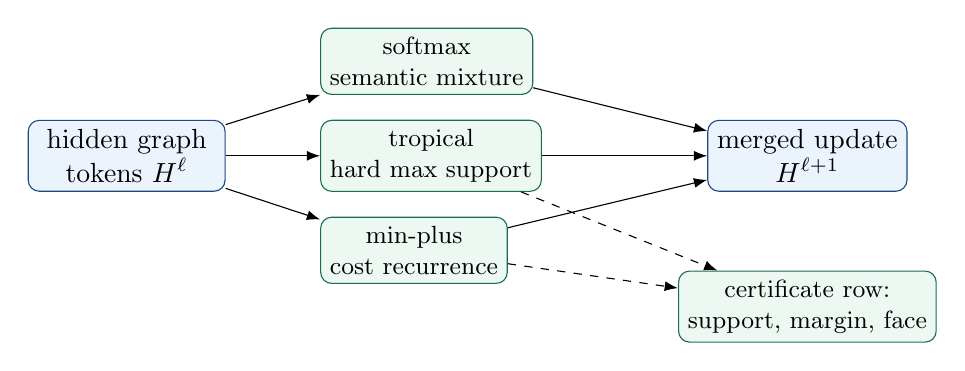
\begin{tikzpicture}[>=Latex,node distance=0.6cm]
\tikzstyle{state}=[draw=darkblue,rounded corners,fill=softblue,align=center,minimum width=2.5cm,minimum height=0.9cm]
\tikzstyle{head}=[draw=darkgreen,rounded corners,fill=softgreen,align=center,minimum width=2.3cm,minimum height=0.8cm,font=\small]
\node[state] (h) {hidden graph\\tokens \(H^\ell\)};
\node[head, right=1.2cm of h, yshift=1.2cm] (soft) {softmax\\semantic mixture};
\node[head, right=1.2cm of h] (trop) {tropical\\hard max support};
\node[head, right=1.2cm of h, yshift=-1.2cm] (min) {min-plus\\cost recurrence};
\node[state, right=2.1cm of trop] (out) {merged update\\\(H^{\ell+1}\)};
\node[head, below=1.0cm of out] (cert) {certificate row:\\support, margin, face};
\draw[->] (h)--(soft); \draw[->] (h)--(trop); \draw[->] (h)--(min);
\draw[->] (soft)--(out); \draw[->] (trop)--(out); \draw[->] (min)--(out);
\draw[->,dashed] (trop)--(cert); \draw[->,dashed] (min)--(cert);
\end{tikzpicture}
\caption{One TropicalGT layer.  Tropical and min-plus heads supply hard supports and dynamic-programming inductive bias; softmax heads retain diffuse semantic modeling.}
\end{figure}

\section{Reasoning trajectories as tropical dynamical objects}

\subsection{Reasoning packets}

A reasoning agent fills a trajectory.  In a graph-token setting, a step is not a sentence but a packet.

\begin{definition}[Tropical reasoning packet]
A tropical reasoning packet at time \(t\) is
\begin{equation}
R_t=(G_t,H_t,U_t,E_t,C_t,A_t,\Gamma_t,B_t),
\end{equation}
where \(G_t\) is a typed graph, \(H_t\) hidden tokens, \(U_t\) retrieved or tool-derived evidence, \(E_t\) verifier fields, \(C_t\) behavior-control coordinates, \(A_t\) active tropical supports, \(\Gamma_t\) fan-cell and margin summaries, and \(B_t\) output bytes or byte logits.  A TropicalGT model induces a stochastic kernel
\begin{equation}
P_\theta(R_{t+1}\mid R_{\le t},x)
\end{equation}
or a deterministic update \(R_{t+1}=F_\theta(R_t,x)\).
\end{definition}

The active supports \(A_t\) are essential.  They say which predecessor, evidence passage, key item, proof clause, or memory block was decisive.  They let the system distinguish a plausible answer from an answer whose internal routing matches a known algorithmic certificate.

\subsection{Tropical trajectory complexes}

From a packet we build a filtered complex.  Let \(V_t\) be tokens and let \(w_t(v)\) be an importance score derived from tropical margins, verifier confidence, evidence scores, or path costs.  For thresholds \(\alpha_0\le\cdots\le\alpha_m\), define
\begin{equation}
K_t(\alpha_p)=\{\sigma\subseteq V_t: \max_{v\in\sigma} w_t(v)\le \alpha_p \text{ and } \sigma \text{ is graph-admissible}\}.
\end{equation}
This produces \(K_t(\alpha_0)\subseteq\cdots\subseteq K_t(\alpha_m)\).  For a path-finding task, low thresholds may include source-connected nodes with low tentative distance; for retrieval, they may include evidence nodes with high tropical support and valid provenance; for behavior control, they may include tone/personality states within a corridor.

\begin{proposition}[Support-stable filtrations]
Suppose the vertex scores \(w_t\) are continuous functions of hidden states and tropical candidate values.  If all active supports used in \(w_t\) have margins at least \(\gamma>0\), then any perturbation of hidden states that changes every candidate value by at most \(\gamma/4\) leaves all active supports unchanged and changes each score by at most a fixed Lipschitz multiple of the perturbation.  Therefore threshold grids with spacing exceeding twice this score perturbation have identical filtration membership.
\end{proposition}
\begin{proof}
Active supports are unchanged by the active support stability theorem.  Conditional on the same support, each score is an affine or smooth local function of the hidden state, hence Lipschitz on the bounded evaluation domain.  If each score changes by less than half the gap between adjacent thresholds, no vertex crosses a threshold, so all simplices have unchanged membership.
\end{proof}

\subsection{Tropical hidden Markov dynamics}

A useful mental model is a finite-state abstraction.  Quantize each packet by its active cell and certificate:
\begin{equation}
q(R_t)=(\text{cell}(H_t), A_t, \Gamma_t, \text{verifier bin}, \text{behavior bin}).
\end{equation}
If the quantization is finite, repeated reasoning induces a Markov chain on certificates.  This permits ergodic diagnostics: occupation of bad behavior chambers, recurrence of low-margin cells, entropy rate of supports, and average bits-per-byte cost per step.

\begin{theorem}[Ergodic average for finite tropical certificate chains]
Let \((Q_t)_{t\ge0}\) be an irreducible aperiodic finite Markov chain induced by quantized TropicalGT reasoning packets, with stationary distribution \(\pi\).  For any bounded certificate observable \(\varphi\),
\begin{equation}
\frac1T\sum_{t=1}^T \varphi(Q_t)\to \sum_q \pi(q)\varphi(q)
\end{equation}
almost surely.  In particular, time-averaged tropical margin, support entropy, verifier error, and bits-per-byte contribution converge to stationary expectations.
\end{theorem}
\begin{proof}
This is the standard strong law for irreducible aperiodic finite Markov chains.  The assumption ensures a unique stationary distribution and positive recurrence.  Applying the Markov-chain ergodic theorem to bounded \(\varphi\) gives the claim.
\end{proof}

This theorem is intentionally modest.  It does not imply a trained model is good.  It says that once the certificate dynamics are finite and stable, empirical time averages are meaningful audit targets.

\section{Dynamic programming simulation and graph reasoning}

\subsection{Bellman recurrences}

Let \(D_t(v)\) be a max-plus value on a directed graph.  The recurrence
\begin{equation}
D_{t+1}(v)=\max\left(D_t(v),\max_{u\to v}\{D_t(u)+w(u,v)\}\right)
\end{equation}
can be implemented by a tropical head with query token \(v\), key set containing \(v\) and incoming neighbors, and value \(D_t(u)+w(u,v)\).  For shortest paths, replace max by min or negate distances.

\begin{theorem}[TropicalGT simulates bounded Bellman-Ford]
Consider a family of directed graphs with at most \(n\) vertices and real edge weights in a bounded interval.  Fix a source \(s\).  There exists a TropicalGT stack with \(O(n)\) min-plus heads per layer and depth \(n-1\) that exactly computes single-source shortest-path distances on graphs with no negative cycles, assuming exact real arithmetic and a mask giving incoming edges.
\end{theorem}
\begin{proof}
The Bellman-Ford recurrence for distances is
\begin{equation}
d_{t+1}(v)=\min\left(d_t(v),\min_{u\to v}\{d_t(u)+w(u,v)\}\right),\qquad d_0(s)=0,
\end{equation}
with \(d_0(v)=+\infty\) for \(v\ne s\).  A min-plus head for each vertex \(v\) masks keys to \(v\) and its incoming neighbors and returns the displayed minimum.  All vertices update in parallel.  After \(n-1\) iterations, Bellman-Ford is exact in graphs without negative cycles because a shortest simple path uses at most \(n-1\) edges.  Thus depth \(n-1\) suffices.
\end{proof}

\subsection{Tropical transitive closure}

Let \(A\in\T^{n\times n}\) be a tropical adjacency matrix.  The finite Kleene star is
\begin{equation}
A^{\star}_{T}=I\oplusT A\oplusT A^{\odotT2}\oplusT\cdots\oplusT A^{\odotT T}.
\end{equation}
It encodes best path weights of length at most \(T\).  Tropical Attention's proof appendix uses the same idea to show that MHTA can learn tropical transitive closure \cite{hashemi2025tropical}.  TropicalGT uses this result in graph-token form.

\begin{corollary}[Graph-token tropical closure]
Given a directed graph with \(n\) valid vertex tokens and a mask for legal edges, a TropicalGT stack with min-plus or max-plus heads can compute horizon-\(T\) path closure using \(T\) layers and \(O(n)\) vertex-parallel heads per layer.  If the task only requires reachability rather than weights, Boolean semiring values can be embedded as \(0\) and \(-\infty\) and computed with max-plus logic.
\end{corollary}

\subsection{Quickselect as active order statistic}

Quickselect asks for the \(k\)-th order statistic.  A tropical head can implement a hard order-statistic certificate by comparing candidates via rank features.  Let \(r_i=\#\{j:x_j\le x_i\}\).  The target token is active when \(|r_i-k|\) is minimal, with tie-breaking by index.  A min-plus head over candidate tokens can compute
\begin{equation}
Y=\min_i\{|r_i-k|+\epsilon i\}.
\end{equation}
The support identifies the selected item.  The training loss should include both classification and support agreement:
\begin{equation}
\calL_{\rm qs}=\operatorname{CE}(\hat y,y)+\lambda_{\rm supp}\operatorname{CE}(\hat A,A^\star)+\lambda_\gamma\max(0,\gamma_0-\gamma).
\end{equation}
The margin term is essential for length generalization: the model should not merely classify correctly at length 8; it should produce a stable support at length 1024.

\subsection{Knapsack as tropical table compression}

For 0/1 knapsack, the dynamic program is
\begin{equation}
D_{i,c}=\max(D_{i-1,c},D_{i-1,c-w_i}+v_i).
\end{equation}
TropicalGT can represent rows of the DP table as tokens and use a tropical head to select between skip and take alternatives.  However, full tables are expensive.  The model should learn compressed table certificates:
\begin{equation}
Z_i=\operatorname{Compress}\{(c,D_{i,c}):c\in[0,C]\},
\end{equation}
where compression may be a set of breakpoints of a piecewise-linear envelope.  The certificate loss compares the envelope rather than all capacities:
\begin{equation}
\calL_{\rm env}=\sum_{c\in\calC_{\rm probe}}\left|\hat D_i(c)-D_i(c)\right|+\lambda_{\rm bp}|\widehat{\operatorname{breakpoints}}|.
\end{equation}
This connects directly to bits-per-byte: a small breakpoint code that predicts future proof or answer tokens is more deployable than a full DP table.

\section{Compression theory: when tropical certificates help bits-per-byte}

TropicalGT uses structural losses only when they reduce future uncertainty or improve reasoning/control without compression regression.  The right mathematical quantity is conditional mutual information.

\begin{definition}[Prequential bits-per-byte]
For a byte sequence \(b_{1:T}\), the prequential bits-per-byte loss is
\begin{equation}
\calL_{\bits}(\theta;b_{1:T})=-\frac1T\sum_{t=1}^T \log_2 p_\theta(b_t\mid b_{<t}).
\end{equation}
The score is valid only when predictions for \(b_t\) depend on prefix-visible information.
\end{definition}

\begin{theorem}[Certificate side-information identity]
Let \(B_t\) be the next byte, \(\calF_t\) the prefix-visible sigma-field, and \(Z_t\) a prefix-visible tropical certificate.  The optimal expected log-loss improvement from observing \(Z_t\) is
\begin{equation}
H(B_t\mid\calF_t)-H(B_t\mid\calF_t,Z_t)=I(B_t;Z_t\mid\calF_t)
\end{equation}
bits.  If storing or computing \(Z_t\) costs \(c_t\) bits amortized per prediction, its net compression utility is positive only if
\begin{equation}
I(B_t;Z_t\mid\calF_t)>c_t.
\end{equation}
\end{theorem}
\begin{proof}
The Bayes-optimal expected log base-2 loss when predicting from \(\calF_t\) is \(H(B_t\mid\calF_t)\).  When \(Z_t\) is also observed, it is \(H(B_t\mid\calF_t,Z_t)\).  Their difference is the definition of conditional mutual information.  A code or artifact costing \(c_t\) bits per prediction improves net compression only when the information gain exceeds the cost.
\end{proof}

This theorem is the central guardrail.  A tropical support is not useful because it is elegant.  It is useful if it lowers entropy of future bytes, selects correct reasoning moves, improves verifier accuracy, or prevents behavior drift at a cost justified by validation.

\begin{definition}[Tropical certificate utility]
For a certificate family \(\calZ\), define
\begin{equation}
U(\calZ)=\Delta\calL_{\bits}^{\rm heldout}+\lambda_A\Delta A+\lambda_R\Delta R+\lambda_C\Delta C-\rho\operatorname{bytes}(\calZ)-\lambda_T\operatorname{time}(\calZ),
\end{equation}
where \(\Delta\calL_{\bits}^{\rm heldout}\) is reduction in held-out bits-per-byte, \(A\) accuracy, \(R\) reasoning quality, and \(C\) control metrics.  A certificate is deployable only if \(U(\calZ)>0\) under matched ablations.
\end{definition}

\section{Losses, metrics, objectives, and regularizers}

This section gives a catalogue of training objectives.  Each item is designed to be implemented first as audit-only, then as a train-time auxiliary, and only later as deployable structure if it survives bits-per-byte accounting.

\subsection{Objective 1: tropical support supervision}

Given a teacher support \(A^\star_{ic}\), minimize
\begin{equation}
\calL_{\rm supp}=\sum_{i,c}\operatorname{CE}(\hat p_{ic},A^\star_{ic}),\qquad \hat p_{ic}=\softmax_j(\beta z_{icj}).
\end{equation}
Although the deployed tropical head is hard, the surrogate uses a high-temperature softmax over candidate values for gradient flow.  This teaches the model \emph{which} evidence or predecessor is decisive.  It is useful for Quickselect, path algorithms, proof-dependency selection, retrieval citation, and tool-output grounding.

\subsection{Objective 2: top-two margin regularization}

For a desired margin \(\gamma_0\), use
\begin{equation}
\calL_{\rm margin}=\E_{i,c}\max(0,\gamma_0-\gamma_{ic}).
\end{equation}
This penalizes fragile decisions.  It should be applied only when labels indicate a deterministic algorithmic step or a high-confidence evidence choice.  In open-ended semantic generation, low margins may correctly represent ambiguity.

\subsection{Objective 3: fan-cell consistency}

For paired examples \((x,x')\) related by graph isomorphism, value shift, or harmless reordering, require active-cell agreement:
\begin{equation}
\calL_{\rm cell}=\operatorname{CE}(\hat c(x),c^\star)+\operatorname{CE}(\hat c(x'),c^\star)+\lambda\mathbf{1}[\hat c(x)\ne\hat c(x')].
\end{equation}
This is a direct regularizer for size and value generalization.  If a shortest-path proof is shifted by adding a constant to all edge costs, the projective cell should not change unless the optimum changes.

\subsection{Objective 4: Hilbert-metric contrastive alignment}

For query \(q\), positive key \(k^+\), and negatives \(k^-\), use
\begin{equation}
\calL_H=\max\left(0,m+d_H(q,k^+)-\min_{k^-}d_H(q,k^-)\right).
\end{equation}
This aligns tropical projective geometry with retrieval or predecessor selection.  It is preferable to Euclidean contrastive loss when global shifts of coordinates should be ignored.

\subsection{Objective 5: Bellman residual loss}

For a task with a known recurrence operator \(T\), define
\begin{equation}
\calL_{\rm Bell}=\sum_t\norm{D_{t+1}-T(D_t)}_1.
\end{equation}
The target \(D_t\) may be a teacher DP table, a compressed envelope, or a hidden projection.  This loss teaches recurrence consistency, not just final-answer accuracy.

\subsection{Objective 6: tropical closure distillation}

Let a teacher compute a closure \(A^\star\) such as all-pairs shortest paths or transitive reachability.  A student predicts \(\hat A\) from one or few MHTA layers:
\begin{equation}
\calL_{\rm closure}=\norm{\hat A-A^\star}_1+\lambda_{\rm tri}\sum_{i,j,k}\max(0,\hat A_{ij}-\hat A_{ik}-\hat A_{kj})
\end{equation}
for min-plus distances.  The triangle penalty enforces metric-like consistency.

\subsection{Objective 7: active-path certificate loss}

For shortest paths, a distance without a predecessor is incomplete.  Let \(\pi^\star(v)\) be the teacher predecessor.  Use
\begin{equation}
\calL_{\rm pred}=\sum_v\operatorname{CE}(\hat\pi(v),\pi^\star(v))+\lambda\sum_v\left|\hat d(v)-\hat d(\hat\pi(v))-w(\hat\pi(v),v)\right|.
\end{equation}
This links the active support to the numeric value.  It prevents a model from predicting correct distances via spurious routes.

\subsection{Objective 8: tropical polynomial sparsity}

For a head with candidates \(r\), encourage small active dictionaries:
\begin{equation}
\calL_{\rm sparse}=\E_x |A(x)|+\lambda\sum_r \sqrt{\E_x \mathbf{1}[r\in A(x)]+\eps}.
\end{equation}
The first term encourages unique active decisions; the second encourages reuse of a compact candidate dictionary.  This improves interpretability and may improve compression by limiting distinct support codes.

\subsection{Objective 9: cell entropy and occupation balance}

Define the empirical distribution of active cells \(\hat p(c)\).  Penalize both collapse and noise:
\begin{equation}
\calL_{\rm occ}=\lambda_{\rm low}\max(0,H_{\min}-H(\hat p))+\lambda_{\rm high}\max(0,H(\hat p)-H_{\max}).
\end{equation}
A model that uses one cell for all examples has not learned algorithmic cases.  A model that uses too many cells may be memorizing.  The useful range is task-specific.

\subsection{Objective 10: soft-to-tropical annealing}

For hybrid heads, train a gate \(g_t\) with schedule
\begin{equation}
\calL_{\rm anneal}=\calL_{\rm task}+\lambda_g\E|g_t-g_t^\star|+\lambda_{\rm KL}\operatorname{KL}(p_{\rm soft}\Vert p_{\rm trop,soft}).
\end{equation}
Early training may rely on softmax for gradients; later training shifts algorithmic steps to tropical heads.  The gate target \(g_t^\star\) is 1 for deterministic recurrence steps and 0 for diffuse semantic steps.

\subsection{Objective 11: tropical Lipschitz robustness}

For adversarial or random perturbations \(\delta\) bounded by \(\norm\delta\le\eps\), use
\begin{equation}
\calL_{\rm rob}=\E_{x,\delta}\norm{f(x+\delta)-f(x)}_1+\lambda\E_{x,\delta}\mathbf{1}[A(x+\delta)\ne A(x)]
\end{equation}
when the label should be invariant.  This objective operationalizes the Hilbert-metric non-expansive intuition.

\subsection{Objective 12: value-shift invariance}

For tasks invariant under adding a constant to all relevant values, train
\begin{equation}
\calL_{\rm shift}=\E_{x,a}\norm{f(x+a{\bf 1})-f(x)}^2+\lambda\operatorname{CE}(A(x+a{\bf 1}),A(x)).
\end{equation}
This exploits tropical projective equivalence.  It is useful for order statistics, argmax tasks, and relative-cost reasoning.

\subsection{Objective 13: tropical retrieval support precision}

For a retrieved context graph, let \(E^\star\) be evidence nodes required by a verifier.  A tropical retrieval head returns support \(A\).  Define
\begin{equation}
\operatorname{Prec}_{\rm trop}=\frac{|A\cap E^\star|}{|A|+\eps},\qquad \operatorname{Rec}_{\rm trop}=\frac{|A\cap E^\star|}{|E^\star|+\eps}.
\end{equation}
Use a differentiable surrogate based on soft supports.  This makes retrieval accountable: the highest tropical evidence should be the evidence used by the answer.

\subsection{Objective 14: graph-of-thought tropical flow conservation}

Let reasoning steps form a DAG.  Let \(F_{uv}\) be tropical flow along edge \(u\to v\).  Enforce
\begin{equation}
\calL_{\rm flow}=\sum_{v\notin\{s,t\}}\left|\max_{u\to v}F_{uv}-\max_{v\to w}F_{vw}\right|.
\end{equation}
In max-plus terms this says the best incoming proof support should match the best outgoing use, except at sources and sinks.  It discourages orphaned claims.

\subsection{Objective 15: tropical contradiction barrier}

For contradictory claim nodes \(a,b\), their simultaneous high support is forbidden:
\begin{equation}
\calL_{\rm contra}=\sum_{(a,b)\in\calR_{\rm contra}}\max(0,s_a+s_b-\tau)^2.
\end{equation}
The tropical version uses \(s_a\oplusT s_b\) and active support; contradictory claims should not both be among top supports of the same proof step.

\subsection{Objective 16: bits-per-byte support utility gate}

For a support code \(Z_t\), estimate conditional utility by a controlled ablation:
\begin{equation}
\widehat\Delta_{\bits}(Z)=\calL_{\bits}(\text{student without }Z)-\calL_{\bits}(\text{student with }Z)-\rho\operatorname{bytes}(Z).
\end{equation}
The code is allowed in deployment only if \(\widehat\Delta_{\bits}(Z)>0\) with confidence under matched seeds.

\subsection{Objective 17: tropical proof-step verifier}

For proof tasks, require each step to have an active predecessor set satisfying a verifier relation:
\begin{equation}
\calL_{\rm proof}=\sum_t\operatorname{CE}(\hat y_t,y_t)+\lambda\sum_t \mathbf{1}[\operatorname{Verifier}(A_t,\text{claim}_t)=0].
\end{equation}
A differentiable proxy scores whether active supports entail the current claim.  The exact verifier runs on sampled batches.

\subsection{Objective 18: context-block max-support stopping}

Let \(M_t\) be the maximum evidence support remaining outside the current context.  Stop when
\begin{equation}
M_t-\max_{j\in\text{context}}S_j<\delta
\end{equation}
and verifier confidence is high.  Train a stopping head with
\begin{equation}
\calL_{\rm stop}=\operatorname{CE}(\hat s_t,s_t^\star)+\lambda \frac{\ell_t}{L_C}.
\end{equation}
This prevents gratuitous long-context expenditure.

\subsection{Objective 19: quantized active-face preservation}

Fake-quantize tropical projections \(\hat Q,\hat K,\hat V\).  Penalize support flips:
\begin{equation}
\calL_{\rm qface}=\E\mathbf{1}[A(Q,K,V)\ne A(\hat Q,\hat K,\hat V)]+\lambda\norm{Y-\hat Y}_1.
\end{equation}
The active support stability theorem gives a margin-based sufficient condition; the loss trains the model to satisfy it.

\subsection{Objective 20: behavior-corridor tropical routing}

Let behavior coordinates include tone, compliance, uncertainty, verbosity, and safety.  For a desired corridor \(K\), define
\begin{equation}
\calL_{\rm beh}=\operatorname{dist}(C_t,K)^2+\lambda\mathbf{1}[A_t\cap A_{\rm unsafe}\ne\emptyset].
\end{equation}
Tropical supports identify the memory, policy, or evidence block that dominated behavior.  The loss is used only with safety and evaluation audits; it should not be optimized blindly.

\subsection{Objective 21: tropical Newton polytope volume control}

Let \(P_h=\Conv\{a_r:r\in A(h)\}\) be the active-face polytope.  Define
\begin{equation}
\calL_{\rm vol}=\E_h \max(0,\operatorname{Vol}(P_h)-V_{\max}).
\end{equation}
Large active faces mean many tied alternatives; this may be appropriate in ambiguous tasks but harmful in deterministic algorithms.  Volume control helps enforce decisive routing.

\subsection{Objective 22: tropical tableau and sorting certificate}

Many order-statistic and scheduling tasks admit Young-tableau-like sorted summaries.  Let \(T(x)\) be a canonical tableau of ranks or intervals.  Train a tropical head to recover row/column predecessor supports:
\begin{equation}
\calL_{\rm tab}=\operatorname{CE}(\hat T,T^\star)+\lambda\sum_{(i,j)}\max(0,T_{i,j}-T_{i,j+1})+\lambda\sum_{(i,j)}\max(0,T_{i,j}-T_{i+1,j}).
\end{equation}
This supplies a combinatorial certificate for sorted reasoning.  It is a bridge between tropical attention and representation-combinatorics.

\subsection{Objective 23: tropical memory recurrence}

For memory retrieval, let \(m_t\) be a memory state and \(z_t\) a retrieved support code.  Train
\begin{equation}
 m_{t+1}=m_t\oplusT (W\odotT z_t),\qquad \calL_{\rm mem}=\norm{\hat m_{t+1}-m_{t+1}^\star}_1+\lambda\operatorname{bytes}(z_t).
\end{equation}
This makes memory update a max-plus accumulation of reusable evidence rather than an unconstrained text append.

\subsection{Objective 24: tropical circuit description length}

Let a task be solved by a learned tropical circuit with \(H\) heads, \(L\) layers, and \(C\) distinct active support patterns.  Define
\begin{equation}
\operatorname{TDL}=\alpha H+\beta L+\rho\log(1+C)+\calL_{\rm task}.
\end{equation}
This is a tropical minimum-description-length objective.  It encourages simple circuits that still solve the task and transfer.

\section{Training paradigms}

\subsection{Paradigm A: drop-in MHTA replacement}

The simplest paradigm is the one used in the Tropical Attention paper: replace every softmax self-attention block in a shallow transformer with MHTA while keeping depth, width, and number of heads comparable.  This is the right first experiment for canonical algorithmic tasks.  TropicalGT uses it as an audit baseline, not necessarily as the final architecture.

\begin{lstlisting}[language=Python,caption={Minimal PyTorch-style tropical head.}]
def tropical_head(X, Wq, Wk, Wv, mask=None, eps=1e-6):
    # X: [B, L, D]
    Q = projective(torch.log(torch.nn.functional.softplus(X @ Wq) + eps))
    K = projective(torch.log(torch.nn.functional.softplus(X @ Wk) + eps))
    V = X @ Wv
    # Hilbert distance: max(Q-K)-min(Q-K) over feature dimension
    diff = Q[:, :, None, :] - K[:, None, :, :]
    dH = diff.max(dim=-1).values - diff.min(dim=-1).values
    S = -dH
    if mask is not None:
        S = S + mask
    # max-plus aggregation by channel
    Y = (S[:, :, :, None] + V[:, None, :, :]).max(dim=2).values
    support = (S[:, :, :, None] + V[:, None, :, :]).argmax(dim=2)
    return Y, support
\end{lstlisting}

\subsection{Paradigm B: tropical-supervised graph-token training}

When graph structure is known, use graph tokens and certificate labels.  The loss is
\begin{equation}
\calL=\calL_{\rm task}+\lambda_{\rm supp}\calL_{\rm supp}+\lambda_{\rm margin}\calL_{\rm margin}+\lambda_{\rm Bell}\calL_{\rm Bell}.
\end{equation}
This paradigm is ideal for shortest paths, reachability, SCC, proof graphs, retrieval citation, and tool-dependency graphs.

\subsection{Paradigm C: teacher-side tropical circuit distillation}

A large teacher runs expensive tropical probes, exact dynamic programs, or long-context ring scans.  It emits compact support codes \(Z\).  A student receives either no code, shuffled code, or real code.  The deployment question is whether real code improves validation after bytes:
\begin{equation}
\calL_{\rm distill}=\operatorname{KL}(p_T(\cdot\mid x)\Vert p_S(\cdot\mid x,Z))+\lambda_Z\operatorname{bytes}(Z)+\lambda_{\bits}\calL_{\bits}.
\end{equation}

\subsection{Paradigm D: tropical retrieval for long context}

In long-context settings, tropical attention is a retrieval and provenance primitive.  Each block \(B_r\) returns a support summary:
\begin{equation}
(m_r,j_r,c_r)=\left(\max_{j\in B_r} z_j,\argmax_{j\in B_r} z_j,\operatorname{code}(B_r)\right).
\end{equation}
The global maximum over blocks gives exact support.  A context filler includes only blocks whose marginal support beats token cost.

\begin{lstlisting}[language=Python,caption={Blockwise tropical retrieval scan.}]
def tropical_block_scan(query, blocks, score_fn, value_fn):
    best_score = -float("inf")
    best_value = None
    best_ref = None
    summaries = []
    for r, block in enumerate(blocks):
        scores = score_fn(query, block)       # [block_len]
        idx = scores.argmax()
        val = value_fn(block[idx])
        summaries.append((scores[idx], r, idx))
        if scores[idx] > best_score:
            best_score = scores[idx]
            best_value = val
            best_ref = (r, int(idx))
    return best_value, best_ref, summaries
\end{lstlisting}

\subsection{Paradigm E: bits-per-byte-gated tropical curriculum}

The recommended training curriculum is:
\begin{enumerate}
\item train a dense baseline with no tropical auxiliaries;
\item add tropical probes audit-only and log supports/margins;
\item turn on support and margin losses for synthetic algorithmic data;
\item add graph-token and retrieval tasks;
\item train a teacher with full tropical certificates;
\item distill compact support codes into a student;
\item export quantized kernels only if bits-per-byte and reasoning gates pass.
\end{enumerate}

\section{Detailed examples}

\subsection{Worked example: a three-node shortest path}

Let vertices be \(s,a,t\) and min-plus edge weights
\begin{equation}
w(s,a)=2,\quad w(a,t)=3,\quad w(s,t)=6.
\end{equation}
Initialize \(d_0(s)=0\), \(d_0(a)=d_0(t)=+\infty\).  After one step:
\begin{align}
d_1(a)&=\min(+\infty,0+2)=2,\\
d_1(t)&=\min(+\infty,0+6)=6.
\end{align}
After two steps:
\begin{equation}
d_2(t)=\min(6,d_1(a)+3)=5.
\end{equation}
The active predecessor support for \(t\) changes from \(s\) to \(a\).  A TropicalGT head should output support \((s\to t)\) at step 1 and \((a\to t)\) at step 2.  The support sequence is a proof certificate: the shortest path is \(s\to a\to t\).  The margin at step 2 is \(6-5=1\); quantization error above \(0.5\) may flip the predecessor, so the active-face preservation theorem gives a concrete bit-precision target.

\subsection{Worked example: subset sum as max-plus reachability}

For weights \(w_1,\ldots,w_n\) and target \(T\), define Boolean reachability \(R_{i,s}\in\{0,-\infty\}\):
\begin{equation}
R_{0,0}=0,
\qquad R_{0,s}=-\infty \text{ for } s\ne0,
\end{equation}
\begin{equation}
R_{i,s}=R_{i-1,s}\oplusT R_{i-1,s-w_i}.
\end{equation}
This is a max-plus recurrence over indicator values.  A tropical head chooses skip or take.  The support path traces the selected subset.  A useful loss is not only \(\operatorname{CE}(\hat R_{n,T},R_{n,T})\) but also a traceback loss comparing selected items.

\subsection{Worked example: proof dependency routing}

Suppose a proof step \(c_t\) depends on either lemma \(\ell_1\) or lemma \(\ell_2\).  The model scores
\begin{equation}
z_j=\operatorname{compat}(c_t,\ell_j)+\operatorname{trust}(\ell_j)+\operatorname{recency}(\ell_j).
\end{equation}
Tropical support chooses \(j^\star=\argmax_j z_j\).  If \(\ell_1\) is correct but \(\ell_2\) is semantically similar and false, softmax may blend them.  Tropical support forces a discrete dependency that can be verified.  The support loss teaches grounded proof routing.

\subsection{Worked example: tone control as tropical corridor selection}

Let behavior states have coordinates \((u,v,w)\): uncertainty, verbosity, warmth.  A policy has chambers:
\begin{align}
C_1&=\{u\le 0.3, v\le0.5\}: \text{concise direct answer},\\
C_2&=\{u>0.3, v\le0.7\}: \text{qualified explanation},\\
C_3&=\{\text{safety risk high}\}: \text{refusal with safe alternative}.
\end{align}
A tropical head selects the chamber by max score.  The behavior-corridor loss penalizes selecting a chamber inconsistent with evidence and safety metadata.  This makes tone and personality control a routing problem with explicit supports rather than an uninspected latent drift.

\section{Implementation and reproducibility}

\subsection{Kernel choices}

The official Tropical Attention repository offers a PyTorch implementation and an optional tropical GEMM backend for max-plus products when available \cite{hashemi2025code}.  A reproducible TropicalGT implementation should support:
\begin{enumerate}
\item pure PyTorch reference kernels;
\item optional CUDA or SIMD max-plus kernels;
\item deterministic support tie-breaking;
\item exact CPU audits on small samples;
\item fake quantization during training;
\item blockwise scans for long context;
\item logging of support ids, margins, and cell ids.
\end{enumerate}

\subsection{Numerical issues}

Tropical heads are stable in one sense and brittle in another.  Output values are Lipschitz with respect to candidate perturbations, but active supports can flip near walls.  This is a feature: walls are exactly where the decision is ambiguous.  Implementation should therefore log both output error and support error.  A model that gets numeric values right but support wrong may be unsuitable for proof or retrieval grounding.

Tie-breaking must be deterministic.  Recommended rule:
\begin{equation}
\argmax^{\rm lex}_j z_j=\min\{j:z_j=\max_k z_k\}.
\end{equation}
For graph data, lexicographic token order must be graph-canonical, not file-order dependent.

\subsection{Quantization}

Let \(b\) be the number of quantization bits and \(\Delta\) the quantization step.  If candidate values are quantized with error at most \(\Delta/2\), then support is preserved whenever margin \(\gamma>\Delta\).  More generally, if scores and values are independently quantized with errors \(\eps_S,\eps_V\), support is preserved when \(\gamma>2(\eps_S+\eps_V)\).  Thus TropicalGT should report the margin distribution before export.  Low-margin heads either need higher precision or must stay teacher-side.

\begin{theorem}[Quantized support preservation]
Let a tropical head have candidate values \(z_j\) and quantized values \(\hat z_j\) satisfying \(|z_j-\hat z_j|\le\eps\) for all \(j\).  If the unique top-two margin is \(\gamma>2\eps\), then \(\argmax_j \hat z_j=\argmax_j z_j\).
\end{theorem}
\begin{proof}
This is the active-support stability theorem with \(\eps_S+\eps_V=\eps\).  The top candidate loses at most \(\eps\) and every competitor gains at most \(\eps\), so the margin remains positive.
\end{proof}

\subsection{Data protocols}

TropicalGT should be evaluated on:
\begin{itemize}
\item canonical combinatorial tasks: Floyd-Warshall, Quickselect, 3SUM, subset sum, balanced partition, convex hull, 0/1 knapsack, fractional knapsack, SCC, bin packing, and minimum coin change, following the Tropical Attention suite;
\item CLRS-style graph algorithm traces;
\item theorem/proof dependency graphs;
\item retrieval-heavy multi-document QA with provenance labels;
\item long-context fill-in tasks with held-out answer bytes;
\item behavior-corridor prompts requiring calibrated tone and uncertainty;
\item mixed natural-language and algorithmic traces where tropical heads should activate only on algorithmic spans.
\end{itemize}

For each dataset, record train length, test length, train value range, test value range, perturbation/noise regime, exact certificate source, and license.  OOD tests must not leak into training.

\subsection{Ablation ladder}

Every result should compare:
\begin{enumerate}
\item softmax transformer baseline;
\item adaptive softmax or sharpened softmax baseline;
\item full tropical replacement;
\item typed hybrid head bank;
\item hybrid plus support supervision;
\item hybrid plus margins and Bellman residual;
\item teacher tropical certificates;
\item distilled compact support codes;
\item quantized deployable model.
\end{enumerate}
Report task accuracy, value error, length OOD, value OOD, perturbation OOD, support accuracy, margin distribution, active-cell entropy, inference time, parameter count, artifact bytes, and held-out bits-per-byte.

\subsection{Reproducibility checklist}

A release should include:
\begin{itemize}
\item exact data-generation scripts and seeds;
\item train/validation/test split hashes;
\item model configs, head types, precision, and masks;
\item kernel backend and version;
\item deterministic tie-breaking mode;
\item exact certificate generator versions;
\item ablation scripts;
\item validation bits-per-byte scorer;
\item support/margin log format;
\item artifact byte accounting script.
\end{itemize}

\section{Theoretical extensions beyond the first iteration}

\subsection{Hybrid softmax-tropical approximation}

A concern is that a purely tropical model may underperform on diffuse semantic tasks.  The following theorem explains why a hybrid bank is not less expressive on bounded domains.

\begin{theorem}[Hybrid head dominance on bounded domains]
Let \(\calF_{\rm soft}\) be functions representable by a fixed softmax transformer family on a compact domain, and \(\calF_{\rm trop}\) functions representable by a fixed tropical transformer family.  A hybrid family with a learned gate and both head types contains \(\calF_{\rm soft}\cup\calF_{\rm trop}\).  If its feed-forward sublayers are universal on the compact token domain, it can approximate finite sums of softmax-representable and tropical-representable components.
\end{theorem}
\begin{proof}
Set the gate identically \(0\) to recover the softmax family and identically \(1\) to recover the tropical family.  For finite sums, route one subset of heads to softmax components and another to tropical components, then use the output projection and feed-forward sublayer to approximate the desired continuous combination on the compact domain.
\end{proof}

\subsection{Tropical softmax limit}

Softmax is related to max by the log-sum-exp limit:
\begin{equation}
\tau\log\sum_j \exp(z_j/\tau)\to\max_j z_j\quad\text{as }\tau\downarrow0.
\end{equation}
But this limit is not the same as using softmax as a stable reasoning primitive.  Gradients and finite-temperature mixtures can blur support.

\begin{lemma}[Log-sum-exp error bound]
For \(z\in\R^n\),
\begin{equation}
\max_j z_j\le \tau\log\sum_j e^{z_j/\tau}\le \max_j z_j+\tau\log n.
\end{equation}
\end{lemma}
\begin{proof}
Let \(M=\max_j z_j\).  Then \(e^{M/\tau}\le\sum_j e^{z_j/\tau}\le n e^{M/\tau}\).  Taking \(\tau\log\) gives the result.
\end{proof}

The error grows with \(\tau\log n\).  Thus fixed-temperature softmax can become increasingly blurry as length grows.  Tropical attention removes the entropy term rather than tuning it.

\subsection{Sparse tropical kernels}

Full tropical attention costs \(O(L^2d)\) if applied densely.  Sparse kernels restrict key sets \(\calN(i)\).  If the true support is contained in \(\calN(i)\), sparse tropical attention is exact.

\begin{proposition}[Sparse support exactness]
Let \(A_{ic}\) be the dense active support.  If \(A_{ic}\subseteq\calN(i)\), then sparse tropical attention over \(\calN(i)\) returns the same output and support as dense tropical attention for \((i,c)\).
\end{proposition}
\begin{proof}
The maximum over all keys is attained inside \(\calN(i)\).  Removing non-active keys cannot change the maximum or its active set.
\end{proof}

This yields an implementation strategy: train a cheap projected retrieval head to propose \(\calN(i)\), then audit support recall.  The tropical head is exact conditional on recall.

\subsection{Tropical retrieval theorem}

Let \(q\) be a query and \(K_j,V_j\) database keys and values.  Suppose a projection \(P\) approximates Hilbert distances:
\begin{equation}
|d_H(q,K_j)-d_H(Pq,PK_j)|\le\eps\quad\text{for all }j.
\end{equation}
If the nearest key has margin \(>2\eps\), projected tropical retrieval returns the same support.

\begin{proof}
The retrieval score is \(-d_H\).  Distance approximation changes every score by at most \(\eps\).  Apply active-support stability.
\end{proof}

This theorem is useful for vector databases.  A learned projection can make search efficient, but the system should report margin-certified support preservation.

\section{Applications}

\subsection{Algorithmic reasoning}

TropicalGT is most naturally suited to tasks where the target computation is a max/min recurrence, a shortest-path closure, an order statistic, a dynamic-programming table, or a greedy choice with exchange proof.  It should be evaluated first on clean synthetic tasks with exact certificates and then on noisy natural variants.

\subsection{Graph reasoning and knowledge graphs}

A knowledge graph query often asks for the best path, most reliable evidence chain, strongest contradiction, or minimal-hop explanation.  Tropical heads are appropriate for path and support selection.  Softmax heads can still summarize multiple semantically related neighbors.  A graph-token model can combine both.

\subsection{MCP and tool reasoning}

Tool calls produce typed records: schema, arguments, output, permission, timestamp, and provenance.  Tropical support can choose the decisive tool output for a reasoning step.  A certificate says: this answer depended on this tool result, not merely on latent memory.

\subsection{Long-context reasoning}

In 1--10M token contexts, dense softmax is not the intended primitive.  Tropical ring scans can identify maximum-support blocks exactly over shards.  The model can then unpack only a small number of high-support blocks.  This is a path toward long-context efficiency: use tropical summaries for hard evidence, then local softmax for detailed reading.

\subsection{Behavior and personality control}

Tone, verbosity, uncertainty, compliance, and safety can be represented as behavior coordinates.  Tropical routing selects behavior chambers based on evidence, task type, and safety metadata.  This is not a replacement for policy or safety evaluation; it is an audit layer that records which context or rule dominated a behavioral choice.

\section{Experimental plan}

\subsection{Hypotheses}

TropicalGT makes five empirical hypotheses:
\begin{enumerate}
\item tropical heads improve length and value OOD on algorithmic tasks;
\item support supervision improves reasoning faithfulness and verifier agreement;
\item margin regularization improves quantized deployment and perturbation robustness;
\item hybrid head banks outperform full tropical replacement on mixed natural/algo tasks;
\item compact support codes can improve held-out bits-per-byte when they are prefix-visible and artifact-cheap.
\end{enumerate}

\subsection{Metrics}

Report:
\begin{itemize}
\item held-out bits-per-byte;
\item in-distribution task accuracy or MSE;
\item length OOD, value OOD, perturbation OOD;
\item support accuracy and support recall;
\item top-two margin quantiles;
\item active-cell entropy;
\item proof/verifier agreement;
\item retrieval support precision/recall;
\item behavior-corridor violation rate;
\item inference time and memory;
\item artifact bytes after export.
\end{itemize}

\subsection{Statistical discipline}

Use matched seeds, paired bootstrap confidence intervals, and an ablation ladder.  A structural metric is not a success criterion alone.  For example, high support accuracy is good only if it transfers to task accuracy, verifier agreement, bits-per-byte, or controllability.

\section{Risks and limitations}

TropicalGT has clear risks.  First, hard support can be wrong.  A wrong hard support may be worse than a soft mixture.  This is why support losses require exact labels or strong teacher certificates.  Second, tropical kernels can be slower than optimized softmax kernels unless sparse or fused.  Third, tropical geometry may encourage overdiscretization of genuinely ambiguous semantic tasks.  Fourth, behavior-corridor routing may be misused if treated as a complete safety system.  Fifth, mathematical certificates can become ornamental unless disciplined by bits-per-byte.

The remedy is not to optimize every objective.  The remedy is staged activation, exact audit, matched ablation, and compression-aware deployment.  Tropical structure should stay teacher-side unless it proves utility.


\section{TropicalGT-I implementation update: graph-token reasoning agent}
\label{sec:tropicalgt-i-implementation-update}

The first implementation pass instantiates the research program above as a compact graph-conditioned reasoning model rather than as a full contest submission.  The implementation target is \texttt{TropicalGT-I}: a TokenGT-style graph tokenizer, a byte-level reasoning language model, a tropical ring attention graph encoder, a GFlowNet trajectory auxiliary, a GraphCG latent-direction auxiliary, and Plotly-based trajectory audits.  This section records the precise methodology so that the paper, code, and reproducibility contract remain synchronized.

\subsection{TokenGT-style graph tokenization}
Each normalized training row is represented as a graph record
\[
  r=(\mathrm{id},x_{\mathrm{text}},q,a,s,G),
\]
where \(q\) is a question, \(a\) an answer, \(s\) a reasoning trace, and \(G=(V,E)\) a typed directed graph.  If the source row lacks \texttt{graph\_json}, the implementation constructs a conservative graph with a problem node, reasoning-step nodes, an answer node, \texttt{depends\_on} edges, and a final \texttt{supports\_answer} edge.  The TokenGT tokenizer follows Kim et al.\ \cite{kim2022tokengt}: it emits a graph token, one token for each vertex, and one token for each valid edge.  Vertex tokens carry endpoint identifiers \((i,i)\); edge tokens carry \((i,j)\); type identifiers distinguish graph, vertex, and edge tokens.  The deterministic identifier map is a finite orthonormal-style coordinate chart with hashed fallback, which is sufficient for the smoke-scale model and preserves the intended equality/incidence tests.

\subsection{Tropical ring attention and certificates}
Given graph-token states \(z_1,\ldots,z_N\in\R^d\), the implemented tropical head computes projected queries, keys, and values and scores token compatibility by negative tropical Hilbert spread,
\[
  S_{ij}=-d^{-1/2}\left(\max_a(q_{ia}-k_{ja})-\min_a(q_{ia}-k_{ja})\right).
\]
The graph context is then a max-plus reduction
\[
  c_{ia}=\max_j\{S_{ij}+v_{ja}\},
\]
followed by a learned linear output map.  The head returns the active support \(\argmax_j S_{ij}\), the top-two margin, and support entropy.  Blockwise evaluation is exact because the maximum over context shards equals the maximum over their maxima.  The v1 implementation logs these quantities as certificate diagnostics: masked support entropy, soft support entropy used by the entropy regularizer, margin mean/min/p05, margin-threshold wall-hit rate, support-boundary rate, structural edge-certificate agreement, and graph/node/edge token counts.

\subsection{Embedding-space Graph-of-Thought GFlowNet training}
Graph-of-Thought reasoning \cite{besta2024got} is internalized as a stochastic process over pooled graph-token states.  A lightweight policy \(\pi_\theta(a\mid h_t)\) samples a small discrete action vocabulary representing expand, merge, refine, stop, retrieve, verify, compress, and reject moves.  The first implementation uses trajectory balance from the continuous GFlowNet theory of Lahlou et al.\ \cite{lahlou2023continuousgfn},
\[
  \mathcal L_{\mathrm{TB}}=\E_\tau\left[\left(\log Z_\theta+\sum_t\log\pi_\theta(a_t\mid h_t)-\log R(\tau)\right)^2\right],
\]
with a smoke-stage reward derived from likelihood improvement and tropical-margin stability.  Later runs can replace this proxy with verifier scores, answer exactness, retrieval provenance, and certificate validity without changing the interface.

At inference time the same action vocabulary defines a bounded test-time scaling controller.  Starting from the prompt graph, TropicalGT scores a frontier of graph-of-thought candidates by a deployment proxy
\[
  S(\tau)=-\operatorname{NLL}(\tau)+\lambda_m \bar m(\tau)+\lambda_\pi \max_a\pi_\theta(a\mid h_\tau)-\lambda_c |T_\tau|,
\]
where \(\bar m(\tau)\) is the mean tropical top-two margin and \(|T_\tau|\) is the graph-token budget.  The controller expands only the top \(w\) candidates for depth \(d\), using the highest-probability GFlowNet actions as branches.  This does not assert that the smoke model has learned a strong verifier; rather, it makes the scaling rule explicit and auditable.  Each candidate records its action path, NLL proxy, tropical support trace, GFlowNet action probabilities, GraphCG direction diagnostics, token budget, and filtered simplicial object, so longer experiments can swap in stronger rewards without changing the report format.

\subsection{GraphCG latent steering}
The GraphCG auxiliary follows Liu et al.\ \cite{liu2024graphcg}: learned directions \(d_1,\ldots,d_m\) define steerable latent edits in pooled graph state space.  The implementation uses a same-condition contrastive term over direction-shifted states, plus orthogonality and sparsity penalties.  This regularizer is intentionally light: it should organize the latent chart in which graph-of-thought trajectories move, not dominate the byte/reasoning objective.

\subsection{Training, evaluation, inference, and visualization contract}
The runnable contract is implemented by six scripts: \texttt{train\_tropicalgt\_i.py}, \texttt{eval\_tropicalgt\_i.py}, \texttt{infer\_tropicalgt\_i.py}, \texttt{validate\_tropicalgt\_i.py}, \texttt{render\_reasoning\_visualizations.py}, and \texttt{audit\_tropicalgt\_i\_readiness.py}.  Data-backed configurations require the moved ToricGT parquet shards explicitly: the loader first builds a row-group metadata index for the train, validation, and test splits, reads examples through a bounded row-group cache rather than concatenating the full corpus into memory, and refuses to fall back to fixtures when \texttt{require\_data} is enabled.  Long-run configurations use a row-group-aware chunk-shuffle sampler that randomizes parquet row-group order while preserving row-group-local reads, avoiding the cache thrashing that would be induced by full random access over multi-million-row shard collections.  The validation script emits this parquet manifest together with graph-token statistics, graph-json fallback rate, node/edge statistics, and sample graph-token descriptors before long training begins.  The readiness audit script combines environment/package checks, required-data manifest checks, sample TokenGT conversion, paper artifact checks, checkpoint reload, finite evaluation, bounded inference scaling, and optional visualization generation into a single JSON/Markdown proof bundle.  Training reports language-model NLL, BPB proxy, GFlowNet trajectory-balance loss, GraphCG contrastive and geometry terms, finite graph-certificate loss and agreement, tropical support entropy, tropical margins, wall-hit rate, graph-token statistics, graph-json fallback rate, examples/sec, tokens/sec, GPU memory, and step throughput to W\&B when enabled.  The first finite certificate objective is deliberately modest: an edge token is structurally certified when its active tropical support is the edge token itself or one of its endpoint vertex tokens.  This is a TokenGT skeleton certificate rather than a semantic proof; it should be promoted only when it improves held-out BPB, verifier score, support faithfulness, or downstream reasoning metrics.  Checkpoints store model state, optimizer state, step, metric history, config, and random-number-generator state; long runs can resume from either the final checkpoint or a periodic \texttt{.latest.pt} checkpoint.  Evaluation reports aggregate NLL/BPB together with optional per-record NLL, tropical support histograms, graph-token traces, and filtered simplicial objects.  Inference emits the generated byte-level argmax string plus tropical support/margin diagnostics, GFlowNet action probabilities, GraphCG direction summaries, a graph-token trace, the filtered object for the prompt graph, and an optional bounded inference-scaling report containing all expanded candidates and the selected graph-of-thought path.  The visualization script projects pooled graph reasoning states by PCA and writes two interactive HTML audits: a three-dimensional embedding trajectory and a two-dimensional PCA plane with NLL as the third coordinate.  It also writes a metric dashboard and a JSON payload containing hover text, PCA/NLL coordinates, and the complete finite filtered simplicial object attached to each plotted point.  In the first implementation this object contains vertices as \(0\)-simplices, graph edges as \(1\)-simplices, directed length-two reasoning paths as \(2\)-simplices, filtration thresholds, and a compact summary; longer runs can replace the deterministic smoke filtration with learned margin, verifier, or persistence-based weights.

This implementation deliberately omits toric-only mechanisms from the ToricGT paper unless they admit a tropical meaning.  Ported methods are the dataset schema, graph-of-thought trajectory view, GFlowNet branch training, GraphCG steering, W\&B discipline, reproducibility reports, and latent-trajectory visual audits.  Omitted methods include noncommutative toric phase memory, toric ideals, and torus-specific chamber constraints; tropical replacements are active faces, Hilbert margins, max-plus supports, and fan-cell certificates.

\section{Conclusion}

Tropical Attention showed that replacing softmax with max-plus projective attention can restore sharp, scale-invariant, polyhedral reasoning for combinatorial tasks.  TropicalGT extends this insight into a broader reasoning-agent methodology.  It treats tropical heads as auditable dynamic-programming primitives, active supports as finite certificates, margins as stability witnesses, Newton polytopes as decision geometry, graph tokens as equivariant carriers, and bits-per-byte as the deployment arbiter.  The resulting program is both mathematical and pragmatic: prove exact statements for finite structures; train with explicit support, margin, recurrence, and certificate losses; and keep only what improves held-out compression or reasoning quality.

\newpage
\appendix
\section{Appendix A: additional proofs}

\subsection{Proof of finite tropical circuit simulation}

\begin{definition}[Layered tropical circuit]
A layered tropical circuit is a finite directed acyclic graph whose input gates are variables or constants and whose internal gates compute either \(u\oplusT v=\max(u,v)\) or \(u\odotT v=u+v\).  Edges go from layer \(\ell\) to layer \(\ell+1\).
\end{definition}

\begin{theorem}[TropicalGT realizes finite layered tropical circuits]
Let \(C\) be a layered tropical circuit of depth \(L\), width at most \(W\), and real constants in a bounded set.  There is a TropicalGT stack of depth \(L+O(1)\), width polynomial in \(W\), and tropical heads polynomial in \(W\), that computes the same circuit on bounded inputs in exact real arithmetic.
\end{theorem}
\begin{proof}
Represent each circuit gate at layer \(\ell\) by a token channel.  A sum gate \(u+v+c\) is computed by an affine feed-forward map because ordinary addition is available in the Euclidean residual stream and also equals tropical multiplication.  A max gate \(\max(u+c_1,v+c_2)\) is computed by a tropical head with two candidate keys whose values are \(u+c_1\) and \(v+c_2\).  Gates in the same layer are independent and can be computed in parallel by separate channels or heads.  Proceed by induction over layers.  The input layer is represented exactly by token values.  If layer \(\ell\) is represented exactly, the above constructions represent every gate in layer \(\ell+1\) exactly.  After \(L\) steps the outputs are represented exactly.
\end{proof}

\subsection{Approximate version under smooth devaluation}

If the tropical output is passed through a smooth devaluation map \(\delta\), exact equality is lost.  On a compact domain, any fixed smooth map is Lipschitz.  Thus if tropical computation is \(\eps\)-accurate before devaluation, the Euclidean output is \(L_\delta\eps\)-accurate after devaluation.  This gives an immediate approximation theorem for practical architectures.

\section{Appendix B: implementation recipes}

\subsection{Tropical Hilbert distance kernel}

\begin{lstlisting}[language=Python]
def hilbert_distance(Q, K):
    # Q: [B,H,Lq,D], K: [B,H,Lk,D]
    diff = Q[:, :, :, None, :] - K[:, :, None, :, :]
    return diff.max(-1).values - diff.min(-1).values
\end{lstlisting}

\subsection{Support and margin logging}

\begin{lstlisting}[language=Python]
def support_and_margin(scores):
    # scores: [B,H,Lq,Lk,C] or [B,H,Lq,Lk]
    top2 = torch.topk(scores, k=2, dim=-1).values
    support = torch.argmax(scores, dim=-1)
    margin = top2[..., 0] - top2[..., 1]
    return support, margin
\end{lstlisting}

\subsection{Fake quantization audit}

\begin{lstlisting}[language=Python]
def fake_quantize(x, bits=8, clip=6.0):
    levels = 2 ** bits - 1
    x = x.clamp(-clip, clip)
    scale = levels / (2 * clip)
    q = torch.round((x + clip) * scale) / scale - clip
    return q

with torch.no_grad():
    y, supp = tropical_head(X, Wq, Wk, Wv, mask)
    yq, suppq = tropical_head(fake_quantize(X), fake_quantize(Wq),
                              fake_quantize(Wk), fake_quantize(Wv), mask)
    support_flip_rate = (supp != suppq).float().mean()
    value_error = (y - yq).abs().mean()
\end{lstlisting}

\section{Appendix C: objective card table}

\begin{longtable}{p{0.06\textwidth}p{0.25\textwidth}p{0.30\textwidth}p{0.30\textwidth}}
\toprule
ID & Objective & Main signal & Deployment rule\\
\midrule
1 & Support supervision & active predecessor/evidence agreement & keep only if support code improves bytes or verifier\\
2 & Margin regularization & stability to quantization/noise & requires margin audit\\
3 & Fan-cell consistency & OOD invariance & deploy as cell code only if compressed\\
4 & Hilbert contrastive & projective retrieval geometry & compare against cosine retrieval\\
5 & Bellman residual & recurrence correctness & teacher-side unless distilled\\
6 & Closure distillation & all-pairs/path closure & compact closure code only\\
7 & Active path & predecessor proof & useful for citation/proof tasks\\
8 & Polynomial sparsity & small candidate dictionary & improves artifact size\\
9 & Cell entropy & avoid collapse/memorization & metric, rarely loss in deployment\\
10 & Annealing & soft-to-hard curriculum & training-only\\
11 & Robustness & perturbation stability & deploy if value OOD improves\\
12 & Shift invariance & projective consistency & cheap augmentation\\
13 & Retrieval support & evidence precision/recall & deploy if retrieval improves\\
14 & Flow conservation & graph-of-thought consistency & verifier-facing\\
15 & Contradiction barrier & incompatible supports & safety/evidence audit\\
16 & Bits-per-byte gate & compression utility & mandatory\\
17 & Proof verifier & support entails claim & proof tasks only\\
18 & Stopping support & minimal context length & long-context deployment\\
19 & Quantized faces & export stability & mandatory for quantized heads\\
20 & Behavior routing & tone/safety chamber & deploy only with safety audits\\
21 & Polytope volume & tied alternative control & task-specific\\
22 & Tableau certificate & rank/sorting combinatorics & useful for order tasks\\
23 & Memory recurrence & max-plus memory update & retrieval/memory tasks\\
24 & Circuit description length & simple tropical circuits & model selection\\
\bottomrule
\end{longtable}

\section{Appendix D: reproducible experimental command sketch}

\begin{lstlisting}[language=bash]
# 1. Generate deterministic data
python scripts/generate_task.py --task floyd_warshall --n_train 8 \
  --n_test 16 32 64 --value_range 0 10 --seed 1 --out data/fw

# 2. Train baseline
python train.py --config configs/softmax.yaml --data data/fw --seed 1

# 3. Train tropical head model
python train.py --config configs/tropicalgt.yaml --data data/fw --seed 1 \
  --log_supports --log_margins

# 4. Run exact audit
python audit.py --ckpt runs/tropicalgt/seed1.pt --data data/fw/test_64 \
  --metrics task support margin value_ood length_ood perturbation

# 5. Quantize and score held-out bytes
python export_quantized.py --ckpt runs/tropicalgt/seed1.pt --bits 8
python score_bits_per_byte.py --artifact export/model.bin --heldout heldout.bytes
\end{lstlisting}

\newpage

\newpage
\section{Appendix E: extended TropicalGT objective cards}

This appendix gives implementation-facing objective cards. They are intentionally more operational than the main text. Each objective begins teacher-side, runs as an audit, and is promoted only when held-out bits-per-byte, verifier accuracy, support recall, context efficiency, or behavior-control metrics improve under matched ablations.

\subsection{Objective 25: tropical support conditional information}
Let $A_t$ be the active support certificate of a tropical head at time $t$, and let $B_{t+1}$ be the next byte or graph token. Define
\begin{equation}
U_{\rm supp}=I(B_{t+1};A_t\mid \calF_t)-\lambda\operatorname{bits}(A_t).
\end{equation}
The empirical estimator uses two predictors, one with and one without the support certificate:
\begin{equation}
\widehat I=\frac1T\sum_t \log_2 q_\phi(B_{t+1}\mid \calF_t,A_t)-\log_2 q_\psi(B_{t+1}\mid \calF_t).
\end{equation}
The goal is not high support entropy. High support entropy can indicate unstable reasoning. The goal is support information that predicts future bytes, verifier outcomes, or valid reasoning moves. In graph tasks this separates useful active predecessors from decorative attention visualizations.

\begin{proposition}[Support utility decomposition]
If $A_t$ is prefix-visible and both predictors are Bayes optimal, then the expected log-score improvement from revealing $A_t$ equals $I(B_{t+1};A_t\mid\calF_t)$ bits.
\end{proposition}
\begin{proof}
The Bayes expected negative log loss without $A_t$ is $H(B_{t+1}\mid\calF_t)$. With $A_t$ it is $H(B_{t+1}\mid\calF_t,A_t)$. Their difference is the conditional mutual information.
\end{proof}

\subsection{Objective 26: min-plus verifier distance}
Given a verifier graph whose nodes are proof obligations and whose edges are admissible proof refinements, let $d_t(v)$ be the min-plus distance from the current reasoning state to obligation $v$. A TropicalGT verifier head predicts
\begin{equation}
\hat d_{t+1}(v)=\min\left(\hat d_t(v),\min_{u\to v}\{\hat d_t(u)+\hat w(u,v)\}\right).
\end{equation}
Train with
\begin{equation}
\calL_{\rm vdist}=\sum_v \rho_v |\hat d_T(v)-d_T^\star(v)|+\lambda\sum_t \operatorname{TV}(\hat d_{t+1}-\hat d_t).
\end{equation}
The distance target can be generated from exact proof graphs, rubric decompositions, or oracle trajectory classifiers. Compression improves when proof obligations become reusable dynamic-programming states rather than repeated natural-language reminders.

\subsection{Objective 27: tropical consistency under graph contraction}
Let $\kappa:G\to G/H$ contract a subgraph $H$ whose internal computation has been summarized by a tropical state vector $s_H$. A contraction-consistent head satisfies
\begin{equation}
F_\theta(G)\simeq \kappa^\ast F_\theta(G/H,s_H).
\end{equation}
Use
\begin{equation}
\calL_{\rm contr}=\|P_\kappa F_\theta(G)-F_\theta(G/H,s_H)\|_2^2+\beta\operatorname{bits}(s_H).
\end{equation}
This is a direct training rule for hierarchical reasoning. If a subproof, tool trace, or retrieved document can be summarized without changing the answer distribution, the context window can use the summary and save tokens.

\subsection{Objective 28: Hilbert-metric calibration}
The Hilbert projective metric is scale-invariant. For two keys $k_i,k_j$, let $d_H(k_i,k_j)$ denote their tropical projective distance. Suppose teacher supports say that two states are equivalent up to tropical scaling. Train
\begin{equation}
\calL_H=\sum_{(i,j)\in P^+}d_H(k_i,k_j)^2+\sum_{(i,j)\in P^-}\max(0,\gamma-d_H(k_i,k_j))^2.
\end{equation}
This objective helps when absolute logit scale is arbitrary but relative tropical order matters. It is especially useful for length extrapolation because dynamic-programming values often grow with sequence length while their projective differences remain stable.

\subsection{Objective 29: support-margin early stopping}
A reasoning trajectory should stop when additional context is unlikely to change the active tropical support or verifier outcome. Define the support margin
\begin{equation}
\Gamma_t=\min_{i,c}\bigl(z^{(1)}_{ic,t}-z^{(2)}_{ic,t}\bigr)
\end{equation}
and predicted answer entropy $H_t$. Train a stopping head with
\begin{equation}
\calL_{\rm stop}=\operatorname{CE}(\hat s_t,s_t^\star)+\lambda\max(0,\gamma-\Gamma_t)\hat s_t+\mu H_t\hat s_t.
\end{equation}
Stopping with low margin is penalized. Continuing after high-margin, low-entropy convergence is penalized by context-length cost. This connects tropical stability to efficient bits-per-byte deployment.

\subsection{Objective 30: tropical beam diversity with exact merge}
Let a trajectory sampler produce beams $\tau^1,\ldots,\tau^K$. Each beam has a tropical support path $A(\tau^k)$ and score $R_k$. Diversity is measured by support-path distance,
\begin{equation}
D_{kl}=1-\frac{|A(\tau^k)\cap A(\tau^l)|}{|A(\tau^k)\cup A(\tau^l)|+\eps}.
\end{equation}
Use
\begin{equation}
\calL_{\rm beam}=-\operatorname{LSE}_k R_k+\lambda\sum_{k<l}\max(0,\delta-D_{kl})^2.
\end{equation}
This encourages multiple genuinely different proof or retrieval routes. Exact merge is possible when two beams reach the same tropical state vector because future max-plus recurrence depends only on that state.

\subsection{Objective 31: tropical monotonicity for cumulative evidence}
For verified evidence accumulation, some coordinates should be monotone under additional reliable evidence. Let $e_t$ be a coordinate for verified support. Require
\begin{equation}
\calL_{\rm mono}=\sum_t\max(0,e_t-e_{t+1})^2 r_t,
\end{equation}
where $r_t$ is zero for retractions or contradicted evidence. This improves control because a model should not forget verified evidence unless contradiction, tool invalidation, or permission boundary changes the state.

\subsection{Objective 32: tropical contradiction cut}
Let $C$ be a contradiction graph on claims, with an edge $a\dashv b$ when two claims cannot both be active. If $s_a,s_b$ are tropical support scores, train
\begin{equation}
\calL_{\rm cut}=\sum_{a\dashv b}\max(0,s_a+s_b-\eta)^2.
\end{equation}
The loss is a max-plus analogue of a cut constraint. It is useful for retrieval-heavy agents where incompatible memories can be retrieved together.

\subsection{Objective 33: parametric tropical curriculum}
For a synthetic problem family indexed by length $n$, value scale $B$, and graph density $p$, train a curriculum distribution $\pi_\alpha(n,B,p)$. The controller increases difficulty when support recall and bits-per-byte pass thresholds:
\begin{equation}
\alpha_{t+1}=\alpha_t+\eta\nabla_\alpha\bigl[\operatorname{Acc}_{\rm OOD}-\lambda\operatorname{bits-per-byte}_{\rm val}\bigr].
\end{equation}
This objective separates interpolation difficulty from algorithmic extrapolation. A model is not credited for solving large instances if its active supports no longer match exact dynamic-programming supports.

\subsection{Objective 34: tropical explanation compression}
An explanation is a compressed certificate $Z$ for a reasoning trajectory. Train a variational code with
\begin{equation}
\calL_{\rm expl}=-\log q_\theta(y\mid x,Z)+\lambda |Z|+\mu\operatorname{CE}(\hat A(Z),A^\star).
\end{equation}
The certificate may contain active predecessor ids, margins, recurrence names, and verified terminal states. It is useful only if it improves prediction or auditing at lower byte cost than a full chain-of-thought transcript.

\subsection{Objective 35: tropical Jacobian sparsity}
For a piecewise-linear tropical map $F$, the local Jacobian is a selector matrix plus affine weights on each active region. Estimate it away from ties and penalize
\begin{equation}
\calL_{\rm Jac}=\|J_F\|_{1,\rm off}+\lambda\operatorname{rank}_\tau(J_F),
\end{equation}
where $\operatorname{rank}_\tau$ is a soft threshold rank proxy. This encourages decisions that depend on few relevant predecessors, improving interpretability and retrieval locality.

\subsection{Objective 36: tropical oracle agreement}
Combine TropicalGT with oracle trajectory classifiers. Let $o_\omega(\tau)$ classify a trajectory by accuracy, tone, compliance, grounding, and efficiency. Let $A(\tau)$ be the tropical support path. Train
\begin{equation}
\calL_{\rm oracle}=\operatorname{CE}(o_\omega(\tau),y_{\rm prop})+\lambda\|r_\phi(A(\tau))-o_\omega(\tau)\|_2^2.
\end{equation}
When support paths predict bad behavior before the final answer, the controller can intervene early by changing retrieval, asking for verification, or projecting the trajectory into a safer behavior corridor.

\newpage
\section{Appendix F: detailed implementation protocol}

\subsection{Data schema}
A reproducible TropicalGT record is a JSON, msgpack, or Arrow object with these fields:
\begin{enumerate}
\item \texttt{id}: stable hash of task instance, generator, and split;
\item \texttt{graph}: node table, edge table, masks, typed attributes, and adjacency indices;
\item \texttt{tokens}: optional natural-language prefix and byte target;
\item \texttt{recurrence}: exact tropical, min-plus, max-plus, Boolean, or log-semiring recurrence name;
\item \texttt{oracle\_states}: exact dynamic-programming states for small instances or sampled states for large instances;
\item \texttt{supports}: active predecessor sets, tie sets, and margins;
\item \texttt{certificates}: optional toric, persistence, sheaf, or commutative-algebra summaries;
\item \texttt{splits}: family id, size id, value-scale id, and leakage-resistant split id.
\end{enumerate}
Every field used by a deployment loss must be prefix-visible at the time it is consumed. If a field uses the target answer or future bytes, it is teacher-only and cannot be used in prequential scoring.

\subsection{Reference training loop}
\begin{lstlisting}[language=Python]
for batch in loader:
    graph = tokenize_graph(batch.graph)
    prefix = tokenize_bytes(batch.prefix)
    H = model.encode(graph, prefix)
    Y, support, margin = model.tropical_heads(H, return_support=True)
    loss = bits_per_byte_loss(model, batch.target_bytes)
    certs = certificate_cache.lookup(batch.ids)
    for family in active_families:
        if controller.enabled(family):
            loss = loss + controller.weight(family) * family.loss(H, Y, support, certs)
    loss.backward()
    optimizer.step()
    if step % audit_interval == 0:
        logs = exact_support_audit(model, batch, certs)
        controller.update(logs, validation_bits_per_byte())
\end{lstlisting}

\subsection{Kernel choices}
The dense tropical kernel is a reference implementation, not the intended long-context kernel. Practical kernels use one of four strategies.
\begin{enumerate}
\item Block scan: compute exact maxima within blocks, then reduce block maxima.
\item Sparse candidate sets: use retrieval to propose $\calN(i)$, then audit support recall.
\item Hybrid soft-tropical: reserve tropical heads for hard dynamic-programming channels and use softmax for semantic interpolation.
\item Quantized tropical: fake-quantize keys and values; promote only if active supports are stable under round trip.
\end{enumerate}

\begin{theorem}[Quantized support preservation]
Let $z_j=S_{ij}+V_{jc}$ have unique maximizer $j^\star$ and margin $\gamma=z_{j^\star}-\max_{j\ne j^\star}z_j$. If quantization perturbs every $z_j$ by at most $\eps<\gamma/2$, then the quantized tropical head has the same active support.
\end{theorem}
\begin{proof}
For any $j\ne j^\star$, the perturbed gap is at least $\gamma-2\eps>0$. Hence $j^\star$ remains strictly maximal.
\end{proof}

\subsection{Reproducibility grid}
Report at least the following grid.
\begin{center}
\begin{tabular}{lll}
\toprule
Axis & Values & Reported metrics\\
\midrule
length & train, 2x, 4x, 8x & accuracy, support recall, bits-per-byte\\
value scale & train, 2x, 8x & margin, verifier error, calibration\\
graph size & train, 2x, 4x & runtime, memory, exactness\\
context budget & 16k, 128k, 1M, 10M & marginal utility, stopping length\\
quantization & fp32, bf16, int8, int4 & support stability, exported bits-per-byte\\
\bottomrule
\end{tabular}
\end{center}

\newpage
\section{Appendix G: ablation suites and failure-mode diagnostics}

\subsection{Ablation philosophy}
TropicalGT should be evaluated by a ladder, not by a single full-model comparison. The ladder is: dense Transformer baseline; graph-token baseline with ordinary softmax heads; hybrid model with tropical heads disabled but probes logged; tropical heads enabled on synthetic dynamic-programming channels only; tropical heads enabled on retrieval and verifier channels; support-supervised teacher; distilled student; full bits-per-byte and behavior audit. A component is credited only if it beats the immediate predecessor under matched seeds, data, training tokens, parameter budget, and artifact-byte accounting.

\subsection{Support faithfulness audit}
A tropical support is faithful when it identifies the actual finite certificate responsible for the output. For a shortest-path instance, the support should be the active predecessor edge. For knapsack, it should be the include/exclude predecessor cell. For retrieval, it should be a graph path to evidence or memory. Define
\begin{equation}
P_{\rm supp}=\frac{|A_\theta\cap A^\star|}{|A_\theta|+\eps},\qquad
R_{\rm supp}=\frac{|A_\theta\cap A^\star|}{|A^\star|+\eps}.
\end{equation}
Report these separately from answer accuracy. A model can answer correctly while using an unfaithful support, especially when dataset artifacts leak shortcuts.

\subsection{Length and scale extrapolation audits}
For every task family, choose training lengths $n\in[n_{\min},n_{\max}]$ and evaluate on $2n_{\max},4n_{\max},8n_{\max}$. Report
\begin{equation}
\Delta_{\rm len}(m)=\operatorname{Acc}(mn_{\max})-\operatorname{Acc}(n_{\max}),\qquad m\in\{2,4,8\}.
\end{equation}
For numerical dynamic-programming tasks, also increase weights or capacities while holding graph size fixed. Define the scale-regret curve
\begin{equation}
R_{\rm scale}(B)=\calL(B)-\calL(B_{\rm train}).
\end{equation}
Report this for accuracy loss, support error, and bits-per-byte. The useful target is stable extrapolation across scales seen in practical algorithmic tasks, not infinite numeric generalization.

\subsection{Retrieval audit}
For memory and MCP settings, exact support labels are often unavailable. Use synthetic graph databases where the evidence path is known, and natural databases where evidence is approximated by citations, tool-call provenance, or manual labels. Report candidate recall, tropical path recall, answer grounding, and context efficiency. Low candidate recall indicates a retrieval-projection failure. High candidate recall but low tropical path recall indicates a tropical scorer failure. High path recall but low grounding indicates a decoder or verifier failure.

\subsection{Behavior audit}
Behavior controls should not be evaluated only by classifier scores. A tone or compliance classifier can be gamed by superficial phrasing. The TropicalGT behavior audit pairs every classifier label with a structural state: evidence strength, support margin, permission boundary, contradiction mass, and uncertainty entropy. A calibrated model should have monotone relations between assertiveness and evidence margin, and refusal strength should increase with permission or safety boundary scores.

\begin{longtable}{p{0.20\textwidth}p{0.32\textwidth}p{0.38\textwidth}}
\toprule
Failure & Symptom & Corrective action\\
\midrule
Softmax leakage & attention mass spread over irrelevant predecessors & increase tropical head weight or margin loss; audit support recall\\
Tropical brittleness & support changes under tiny perturbations & add margin regularization and tie-aware labels\\
Decorative support & supports are stable but unrelated to exact certificate & train support conditional information; reject if utility is zero\\
Length overfitting & good in-distribution accuracy but poor long length & curriculum on recurrence depth and graph size\\
Scale failure & larger weights break recurrence & Hilbert-metric calibration and projective normalization\\
Retrieval overreach & many context blocks with low utility & marginal context utility gate and contraction summaries\\
Behavior drift & tone changes without evidence-state change & behavior-chart monotonicity and oracle agreement\\
Compression failure & structural module improves task but worsens bits-per-byte & keep teacher-side and distill only support summaries\\
\bottomrule
\end{longtable}

\newpage
\section{Appendix H: additional proofs and worked examples}

\begin{lemma}[Maximum as a nonexpansive operator]
For vectors $a,b\in\R^n$,
\begin{equation}
|\max_i a_i-\max_i b_i|\le \|a-b\|_\infty.
\end{equation}
\end{lemma}
\begin{proof}
For every $i$, $a_i\le b_i+\|a-b\|_\infty$, so $\max_i a_i\le \max_i b_i+\|a-b\|_\infty$. Reversing $a$ and $b$ gives the opposite inequality.
\end{proof}

\begin{theorem}[Tropical recurrence stability]
Consider a recurrence $x_{t+1}=F_t(x_t)$ where every $F_t$ is composed of affine maps with operator norm at most $L$ and coordinatewise maxima. If perturbed maps $\hat F_t$ satisfy $\sup_x\|F_t(x)-\hat F_t(x)\|_\infty\le\eps_t$, then
\begin{equation}
\|x_T-\hat x_T\|_\infty\le \sum_{t=0}^{T-1}L^{T-1-t}\eps_t,
\end{equation}
assuming the same initial state.
\end{theorem}
\begin{proof}
The maximum operator is nonexpansive and the affine parts are $L$-Lipschitz. Thus $F_t$ is $L$-Lipschitz. The error recursion is
\begin{equation}
\|x_{t+1}-\hat x_{t+1}\|_\infty\le L\|x_t-\hat x_t\|_\infty+\eps_t.
\end{equation}
Iterating from zero initial error gives the stated bound.
\end{proof}

\begin{proposition}[Tie-aware supervision is necessary]
If an exact recurrence has a tie set $A^\star$ with more than one maximizer, any single-index cross-entropy target introduces arbitrary symmetry breaking. A set-valued target with uniform mass over $A^\star$ is invariant under relabeling of tied maximizers.
\end{proposition}
\begin{proof}
A single-index target chooses one element of $A^\star$, so permuting two tied maximizers can change the label while leaving the mathematical recurrence unchanged. The uniform distribution on $A^\star$ is fixed by every permutation preserving the set.
\end{proof}

\begin{theorem}[Support recall implies exact sparse output]
Let a dense tropical head compute $Y_{ic}=\max_{j\in J}z_{icj}$. Let $N_i\subseteq J$ be a sparse candidate set. If $A_{ic}=\argmax_{j\in J}z_{icj}\subseteq N_i$, then the sparse head $\max_{j\in N_i}z_{icj}$ has the same value and same active support.
\end{theorem}
\begin{proof}
The dense maximum is attained by every element of $A_{ic}$, and all these elements are included in $N_i$. No element outside $A_{ic}$ exceeds the maximum by definition. Restricting to $N_i$ preserves the maximum value and the maximizers.
\end{proof}

\subsection{Shortest path with active predecessor certificate}
Consider the graph $s\to a\to t$ and $s\to t$ with weights $w(s,a)=2$, $w(a,t)=3$, and $w(s,t)=6$. The min-plus recurrence yields
\begin{align}
d_0(s)&=0,& d_0(a)&=\infty,& d_0(t)&=\infty,\\
d_1(a)&=2,& d_1(t)&=6,\\
d_2(t)&=\min(6,2+3)=5.
\end{align}
The active predecessor for $t$ changes from $s$ to $a$ at the second relaxation. A TropicalGT head should expose support certificate $A_t=\{a\}$ and margin $1$. If a perturbation changes all candidate scores by less than $1/2$, the active predecessor is stable.

\subsection{Subset sum as Boolean tropical reachability}
For weights $2,3,5$ and target $7$, use Boolean tropical values $R_{i,s}\in\{0,-\infty\}$, where $0$ means reachable. Initialize $R_{0,0}=0$ and $R_{0,s}=-\infty$ for $s\ne0$. The recurrence is
\begin{equation}
R_{i,s}=\max(R_{i-1,s},R_{i-1,s-w_i}).
\end{equation}
The target $7$ is reached by $2+5$. The active support certificate for $(i,s)=(3,7)$ points to $(2,2)$, then to $(1,2)$, then to $(0,0)$. This chain is an explanation certificate whose byte cost is logarithmic in the table size if stored as predecessor bits.

\subsection{Tropical retrieval over a knowledge graph}
Suppose a long-context memory graph contains claims $c_i$, tools $u_j$, and evidence nodes $e_k$. A question asks for a claim that depends on evidence nodes and a successful tool call. A retrieval head proposes $\calN(q)$. The tropical verifier computes
\begin{equation}
S(q,c)=\max_{p:q\leadsto c}\sum_{e\in p}w_e+\sum_{u\in p}w_u-\sum_{b\in p}\operatorname{penalty}(b),
\end{equation}
where $b$ ranges over permission or contradiction boundary crossings. The active path becomes the provenance certificate. Training penalizes missing evidence, unsupported citations, and high-scoring paths that cross permission boundaries.

\newpage
\section{Appendix I: deployment and reporting checklist}

A TropicalGT model card should include the following questions and answers. Which heads are tropical, which are softmax, and which are hybrid? Are tropical supports logged during training, validation, or both? Are support labels exact, approximate, or unavailable? What are the in-distribution and out-of-distribution length ranges? What are the value-scale ranges? What is the support recall of sparse retrieval candidate sets? What is the quantized support stability? Which structural losses are teacher-only? Which structural losses survive in the student artifact? What is the held-out bits-per-byte delta after artifact-byte accounting? What are the failure cases where tropical structure hurts? Does behavior control depend on evidence state, or only on style labels?

This checklist makes claims falsifiable. TropicalGT is useful when the structural channels explain and improve the model. If the channels are unfaithful, unstable, or too expensive, they should be removed or left in the teacher stack. The final deployment rule is deliberately conservative. A tropical module may be beautiful, interpretable, and mathematically exact on synthetic examples, yet still fail to improve held-out bits-per-byte on natural text. In that case it remains a teacher-side tool. The deployable student receives only the distilled parts that survive quantized export, support recall audits, and score-first validation.


\begin{thebibliography}{99}

\bibitem{hashemi2025tropical}
Baran Hashemi, Kurt Pasque, Chris Teska, and Ruriko Yoshida.
\newblock Tropical Attention: Neural Algorithmic Reasoning for Combinatorial Algorithms.
\newblock \emph{arXiv:2505.17190}, 2025.

\bibitem{hashemi2025openreview}
Baran Hashemi, Kurt Pasque, Chris Teska, and Ruriko Yoshida.
\newblock Tropical Attention: Neural Algorithmic Reasoning for Combinatorial Algorithms.
\newblock NeurIPS 2025 poster, OpenReview record, 2025.

\bibitem{hashemi2025code}
Baran Hashemi et al.
\newblock \texttt{Baran-phys/Tropical-Attention}: official code for Tropical Attention.
\newblock GitHub repository, 2025.

\bibitem{hashemi2025slides}
Baran Hashemi, Kurt Pasque, Chris Teska, and Ruriko Yoshida.
\newblock Tropical Attention: Neural Algorithmic Reasoning for Combinatorial Algorithms.
\newblock NeurIPS 2025 presentation slides, 2025.

\bibitem{su2026expressivity}
Ye Su and Yong Liu.
\newblock Expressivity of transformers: A tropical geometry perspective.
\newblock \emph{arXiv:2604.14727}, 2026.

\bibitem{schreiber2026tokengtexpressivity}
Amelie Schreiber.
\newblock Expressivity of tokenized graph transformers in terms of tropical geometry, Boolean circuits, and toric fans.
\newblock Local manuscript, 2026.

\bibitem{maclagan2015}
Diane Maclagan and Bernd Sturmfels.
\newblock \emph{Introduction to Tropical Geometry}.
\newblock American Mathematical Society, 2015.

\bibitem{joswig2021}
Michael Joswig.
\newblock \emph{Essentials of Tropical Convexity}.
\newblock American Mathematical Society, 2021.

\bibitem{maragos2021}
Petros Maragos, Vasileios Charisopoulos, and Emmanouil Theodosis.
\newblock Tropical geometry and machine learning.
\newblock \emph{Proceedings of the IEEE}, 109(5):728--755, 2021.

\bibitem{zhang2018}
Liwen Zhang, Gregory Naitzat, and Lek-Heng Lim.
\newblock Tropical geometry of deep neural networks.
\newblock In \emph{Proceedings of ICML}, 2018.

\bibitem{brandenburg2024}
Marie-Charlotte Brandenburg, Georg Loho, and Guido Montufar.
\newblock The real tropical geometry of neural networks for binary classification.
\newblock \emph{Transactions on Machine Learning Research}, 2024.

\bibitem{pasque2024}
Kurt Pasque, Christopher Teska, Ruriko Yoshida, Keiji Miura, and Jefferson Huang.
\newblock Tropical decision boundaries for neural networks are robust against adversarial attacks.
\newblock \emph{arXiv:2402.00576}, 2024.

\bibitem{velickovic2025softmax}
Petar Velickovic, Christos Perivolaropoulos, Federico Barbero, and Razvan Pascanu.
\newblock Softmax is not enough (for sharp size generalisation).
\newblock \emph{arXiv:2410.01104}, 2024/2025.

\bibitem{velickovic2022clrs}
Petar Velickovic, Adri\`a Puigdom\`enech Badia, David Budden, Razvan Pascanu, Andrea Banino, Misha Dashevskiy, Raia Hadsell, and Charles Blundell.
\newblock The CLRS Algorithmic Reasoning Benchmark.
\newblock In \emph{Proceedings of ICML}, 2022.

\bibitem{dudzik2022}
Andrew J. Dudzik and Petar Velickovic.
\newblock Graph neural networks are dynamic programmers.
\newblock In \emph{Advances in Neural Information Processing Systems}, 2022.

\bibitem{vaswani2017}
Ashish Vaswani, Noam Shazeer, Niki Parmar, Jakob Uszkoreit, Llion Jones, Aidan Gomez, Lukasz Kaiser, and Illia Polosukhin.
\newblock Attention is all you need.
\newblock In \emph{Advances in Neural Information Processing Systems}, 2017.

\bibitem{dao2022}
Tri Dao, Daniel Y. Fu, Stefano Ermon, Atri Rudra, and Christopher R\'e.
\newblock FlashAttention: Fast and memory-efficient exact attention with IO-awareness.
\newblock In \emph{Advances in Neural Information Processing Systems}, 2022.

\bibitem{liu2023ring}
Hao Liu, Matei Zaharia, and Pieter Abbeel.
\newblock Ring Attention with blockwise transformers for near-infinite context.
\newblock \emph{arXiv:2310.01889}, 2023.

\bibitem{katharopoulos2020}
Angelos Katharopoulos, Apoorv Vyas, Nikolaos Pappas, and Francois Fleuret.
\newblock Transformers are RNNs: Fast autoregressive transformers with linear attention.
\newblock In \emph{Proceedings of ICML}, 2020.

\bibitem{akian2012}
Marianne Akian, Stephane Gaubert, and Alexander Guterman.
\newblock Tropical polyhedra are equivalent to mean payoff games.
\newblock \emph{International Journal of Algebra and Computation}, 22(1), 2012.

\bibitem{joswig2022shortest}
Michael Joswig and Benjamin Schroeter.
\newblock Parametric shortest-path algorithms via tropical geometry.
\newblock \emph{Mathematics of Operations Research}, 47(3):2065--2081, 2022.

\bibitem{jukna2014}
Stasys Jukna.
\newblock \emph{Tropical Circuit Complexity}.
\newblock In related surveys and monographs on Boolean and tropical circuits, 2014.

\bibitem{gaubert2011}
Stephane Gaubert and Ricardo Katz.
\newblock The Minkowski theorem for max-plus convex sets.
\newblock \emph{Linear Algebra and its Applications}, 2011.

\bibitem{talbut2024}
Roan Talbut, Daniele Tramontano, Yueqi Cao, Mathias Drton, and Anthea Monod.
\newblock Probability metrics for tropical spaces of different dimensions.
\newblock 2024.

\bibitem{nardelli2021}
Nicol\`o Nardelli et al.
\newblock Neural algorithmic reasoning.
\newblock Research program and overview articles, 2021--2025.

\bibitem{cormen2009}
Thomas H. Cormen, Charles E. Leiserson, Ronald L. Rivest, and Clifford Stein.
\newblock \emph{Introduction to Algorithms}.
\newblock MIT Press, 3rd edition, 2009.

\bibitem{floyd1962}
Robert W. Floyd.
\newblock Algorithm 97: Shortest path.
\newblock \emph{Communications of the ACM}, 5(6):345, 1962.

\bibitem{warshall1962}
Stephen Warshall.
\newblock A theorem on Boolean matrices.
\newblock \emph{Journal of the ACM}, 9(1):11--12, 1962.

\bibitem{bellman1958}
Richard Bellman.
\newblock On a routing problem.
\newblock \emph{Quarterly of Applied Mathematics}, 16:87--90, 1958.

\bibitem{ford1956}
Lester R. Ford.
\newblock Network flow theory.
\newblock RAND Corporation, 1956.

\bibitem{knuth1973}
Donald E. Knuth.
\newblock \emph{The Art of Computer Programming, Volume 3: Sorting and Searching}.
\newblock Addison-Wesley, 1973.

\bibitem{cox2011}
David Cox, John Little, and Hal Schenck.
\newblock \emph{Toric Varieties}.
\newblock American Mathematical Society, 2011.

\bibitem{miller2005}
Ezra Miller and Bernd Sturmfels.
\newblock \emph{Combinatorial Commutative Algebra}.
\newblock Springer, 2005.

\bibitem{toricgt1}
Amelie Schreiber.
\newblock ToricGT with Toric BGG Supervision: Graph-Token Reasoning, Hypertoric Category O, and Bits-per-byte-Constrained Training.
\newblock Research manuscript, 2026.

\bibitem{toricgt2}
Amelie Schreiber.
\newblock ToricGT II: Full-Context Dynamical, Ergodic, and Derived Persistence Geometry for Iterative Reasoning Agents.
\newblock Research manuscript, 2026.

\bibitem{toricgt3}
Amelie Schreiber.
\newblock ToricGT III: MCP Memory, Graph-Structured Vector Retrieval, and Long-Context Tropical Ring Attention.
\newblock Research manuscript, 2026.

\bibitem{toricgt4}
Amelie Schreiber.
\newblock ToricGT IV: Oracle Trajectory Classifiers for Behavior, Reasoning Quality, and Bits-per-byte Control.
\newblock Research manuscript, 2026.

\bibitem{west2001}
Douglas B. West.
\newblock \emph{Introduction to Graph Theory}.
\newblock Prentice Hall, 2001.

\bibitem{schrijver2003}
Alexander Schrijver.
\newblock \emph{Combinatorial Optimization: Polyhedra and Efficiency}.
\newblock Springer, 2003.

\bibitem{rockafellar1970}
R. Tyrrell Rockafellar.
\newblock \emph{Convex Analysis}.
\newblock Princeton University Press, 1970.

\bibitem{boyd2004}
Stephen Boyd and Lieven Vandenberghe.
\newblock \emph{Convex Optimization}.
\newblock Cambridge University Press, 2004.

\bibitem{gondran2008}
Michel Gondran and Michel Minoux.
\newblock \emph{Graphs, Dioids and Semirings: New Models and Algorithms}.
\newblock Springer, 2008.

\bibitem{butkovic2010}
Peter Butkovic.
\newblock \emph{Max-linear Systems: Theory and Algorithms}.
\newblock Springer, 2010.

\bibitem{mohri2002}
Mehryar Mohri.
\newblock Semiring frameworks and algorithms for shortest-distance problems.
\newblock \emph{Journal of Automata, Languages and Combinatorics}, 7(3):321--350, 2002.

\bibitem{goodfellow2015}
Ian Goodfellow, Jonathon Shlens, and Christian Szegedy.
\newblock Explaining and harnessing adversarial examples.
\newblock In \emph{International Conference on Learning Representations}, 2015.

\bibitem{hendrycks2021}
Dan Hendrycks and Thomas Dietterich.
\newblock Benchmarking neural network robustness to common corruptions and perturbations.
\newblock \emph{International Conference on Learning Representations}, 2019.

\bibitem{zaheer2017}
Manzil Zaheer et al.
\newblock Deep Sets.
\newblock In \emph{Advances in Neural Information Processing Systems}, 2017.

\bibitem{ying2021}
Chengxuan Ying et al.
\newblock Do Transformers really perform badly for graph representation?
\newblock \emph{Advances in Neural Information Processing Systems}, 2021.

\bibitem{kim2022tokengt}
Jinwoo Kim, Tien Dat Nguyen, Seonwoo Min, Sungjun Cho, Moontae Lee, Honglak Lee, and Seunghoon Hong.
\newblock Pure Transformers are powerful graph learners.
\newblock \emph{Advances in Neural Information Processing Systems}, 2022.

\bibitem{grathwohl2021}
Will Grathwohl et al.
\newblock Backpropagation through the void: Optimizing control variates for black-box gradient estimation.
\newblock Related estimator methodology, 2021.

\bibitem{paszke2019}
Adam Paszke et al.
\newblock PyTorch: An imperative style, high-performance deep learning library.
\newblock In \emph{Advances in Neural Information Processing Systems}, 2019.

\bibitem{harris2020}
Charles R. Harris et al.
\newblock Array programming with NumPy.
\newblock \emph{Nature}, 585:357--362, 2020.

\bibitem{pedregosa2011}
Fabian Pedregosa et al.
\newblock Scikit-learn: Machine learning in Python.
\newblock \emph{Journal of Machine Learning Research}, 12:2825--2830, 2011.


\bibitem{besta2024got}
Maciej Besta, Nils Blach, Ales Kubicek, Robert Gerstenberger, Michal Podstawski, Lukas Gianinazzi, Joanna Gajda, Tomasz Lehmann, Hubert Niewiadomski, Piotr Nyczyk, and Torsten Hoefler.
\newblock Graph of thoughts: Solving elaborate problems with large language models.
\newblock In \emph{AAAI}, 2024.

\bibitem{lahlou2023continuousgfn}
Salem Lahlou, Tristan Deleu, Pablo Lemos, Dinghuai Zhang, Alexandra Volokhova, Alex Hernandez-Garcia, Lena Nehale Ezzine, Yoshua Bengio, and Nikolay Malkin.
\newblock A theory of continuous generative flow networks.
\newblock In \emph{International Conference on Machine Learning}, 2023.

\bibitem{liu2024graphcg}
Shengchao Liu, Chengpeng Wang, Jiarui Lu, Weili Nie, Hanchen Wang, Zhuoxinran Li, Bolei Zhou, and Jian Tang.
\newblock Unsupervised discovery of steerable factors when graph deep generative models are entangled.
\newblock \emph{Transactions on Machine Learning Research}, 2024.

\end{thebibliography}

\end{document}
